%	REQUIRED PACKAGE  %----------------------------------------------------------------------
\documentclass[12pt]{report}
\usepackage[numbers,sort&compress]{natbib}
\usepackage[utf8]{inputenc}
\usepackage{amsmath,amsfonts,amssymb}
\usepackage{graphicx}
\usepackage{tikz}
\usepackage{float}
\usepackage{placeins}
\usepackage{url}
\usepackage{caption}
\usepackage{setspace}
\usepackage{tocloft}


\usepackage[english]{babel}
\usepackage{ragged2e}



%----------------------------------------------------------------------
%	FONTS,INDENTATION, MARGINS, LINE SPACING
%----------------------------------------------------------------------
\usepackage{times}      % Loads the Times-Roman Fonts
\usepackage{mathptmx}   % Loads the Times-Roman Math Fonts
\usepackage[left=3.81cm,
            right=2.54cm,
		top=2.54cm,
		bottom=2.54cm,
		a4paper]{geometry}
% \usepackage[left=2.54cm,
%             right=2.54cm,
% 		top=2.54cm,
% 		bottom=2.54cm,
% 		a4paper]{geometry}
  
\setlength{\parindent}{0pt} % Remove paragraph indent globally

\usepackage{setspace} %package for line spacing
\setstretch{1.5}
\usepackage{parskip}
\setlength{\parskip}{6pt}  % Adjust paragraph spacing as needed

%----------------------------------------------------------------------
%	TITLES,SECTIONS,SUBSECTIONS AND SUBSUBSECTIONS
%----------------------------------------------------------------------
\usepackage{titlesec}
\titlespacing{\chapter}{0pt}{-24pt}{12pt}
\titlespacing{\section}{0pt}{16pt}{16pt}
\titlespacing{\subsection}{0pt}{16pt}{16pt}
\titlespacing{\subsubsection}{0pt}{16pt}{16pt}

\titleformat{\chapter}[display]{\centering\fontsize{14pt}{12pt}\bfseries}{\MakeUppercase{\chaptertitlename\ \thechapter}}{12pt}{}


\titleformat{\section}{\fontsize{12pt}{16pt}\bfseries\raggedright}{\thesection}{0.5em}{}
\titleformat{\subsection}{\fontsize{12pt}{16pt}\bfseries\raggedright}{\thesubsection}{0.5em}{}
\titleformat{\subsubsection}{\fontsize{12pt}{16pt}\bfseries\raggedright}{\thesubsubsection}{0.5em}{}
\titleformat{\paragraph}{\fontsize{12pt}{0pt}\bfseries\raggedright}{\theparagraph}{0.5em}{}



%----------------------------------------------------------------------
%	FORMATTING THE TABLE OF CONTENTS,LOF AND LOT
%----------------------------------------------------------------------

% Adjust the spacing for the TABLE OF CONTENT
\renewcommand{\cftbeforetoctitleskip}{-18pt} % Space before the TOC title
\renewcommand{\cftaftertoctitleskip}{12pt} % Space after the TOC title
\renewcommand{\cftbeforechapskip}{9pt} % Space before each chapter entry
\renewcommand{\cftbeforesecskip}{9pt} % Space before each section entry
\renewcommand{\cftbeforesubsecskip}{9pt} % Space before each section entry
\renewcommand{\contentsname}{\fontsize{12}{14}\bfseries TABLE OF CONTENTS}

% Adjust the spacing for the LIST OF FIGURES
\renewcommand{\cftbeforeloftitleskip}{-18pt} % Space before the LOF title
\renewcommand{\cftafterloftitleskip}{12pt} % Space after the LOF title
\renewcommand{\cftbeforefigskip}{10pt} % Space before each figure entry
\renewcommand{\listfigurename}{\fontsize{12}{14}\bfseries LIST OF FIGURES}
\renewcommand{\cftfigpresnum}{\figurename\ }
\renewcommand{\cftfigaftersnum}{:}
\renewcommand{\cftfigaftersnumb}{\hspace{2.5em}} 

% Adjust the spacing for the LIST OF TABLES
\renewcommand{\cftbeforelottitleskip}{-18pt} % Space before the LOT title
\renewcommand{\cftafterlottitleskip}{12pt} % Space after the LOT title
\renewcommand{\cftbeforetabskip}{10pt} % Space before each table entry
\renewcommand{\listtablename}{\fontsize{12}{14}\bfseries LIST OF TABLES}
\renewcommand{\cfttabpresnum}{Table\ }
\renewcommand{\cfttabaftersnum}{:}
\renewcommand{\cfttabaftersnumb}{\hspace{2.5em}}

%----------------------------------------------------------------------
%	END OF PREAMLBE AND BEGINNING OF THE DOCUMENT
%----------------------------------------------------------------------
% \usepackage{fontspec} % If using XeLaTeX or LuaLaTeX

% \usepackage{graphicx}
% \usepackage[final]{microtype}
% \raggedbottom
% \documentclass{article}
% \usepackage{hyphenat}
% \hyphen
% \raggedright
% \usepackage[document]{ragged2e}



% \justifying
\tolerance=1
\emergencystretch=\maxdimen
\hyphenpenalty=10000
\hbadness=10000

\begin{document}

\pagenumbering{roman} % roman page numbers
\begin{titlepage}
    \centering
    
    
\includegraphics[width=0.2\textwidth]{Graphics/TULogo.png}\par
    \vspace{1.2cm}
    {\fontsize{14pt}{12pt}\selectfont\bfseries\textcolor{black}
    TRIBHUVAN UNIVERSITY \par INSTITUTE OF ENGINEERING \par PURWANCHAL CAMPUS \par
    \vspace{1.2cm}
    \begin{flushleft}
    
    \end{flushleft}

    % {\bfseries\textcolor{black}
    \par VOICE CONTROLLED ROBOT WITH COMPUTER VISION AND ROBOTIC ARM \par

    \vspace{1.2cm}
    BY\par ANKITA RAI KHALING (44001)
    \par MAHESH BOGATI (44018)
      \par SANGRAM BHANDARI (44030)
      \par SARTHAK CHAUDARY (44034)
    \par
    \vspace{0.5cm}
    A PROJECT SUBMITTED TO THE DEPARTMENT OF\par ELECTRONICS AND COMPUTER ENGINEERING IN PARTIAL \par FULFILLMENT OF THE REQUIREMENT FOR THE  \par BACHELOR’S DEGREE IN ELECTRONICS COMMUNICATION AND INFORMATION ENGINEERING\par
    \vspace{1.0cm}\par
    }
    {\fontsize{13pt}{12pt}\selectfont\bfseries\textcolor{black}
    DEPARTMENT OF ELECTRONICS AND COMPUTER ENGINEERING\par PURWANCHAL CAMPUS\par DHARAN, NEPAL\par
    MARCH,2024 
    }
\end{titlepage}


\pagenumbering{roman} % roman page numbers
\begin{titlepage}
    \centering
    
    {\fontsize{12pt}{14pt}\bfseries\textcolor{black}{VOICE CONTROLLED ROBOT WITH COMPUTER VISION AND ROBOTIC ARM}\par}
    \vspace{2.0cm}
       {BY}\par {ANKITA RAI KHALING} ({44001})
       \par {MAHESH BOGATI}({44018})
            \par {SANGRAM BHANARI}({44030})
            \par {SARTHAK CHAUDARY}({44034})
       \vspace{2.0cm}\par
    Project Supervisor\par
    Asst. Prof. Rajnish Rajbahak\par
    \vspace{2.0cm}
    {A project submitted to the Department of Electronics and Computer Engineering in partial fulfillment of the requirements for the Bachelor’s Degree in Electronics Communication and information Engineering}\par
        \vspace{2.0cm}\par

    {Department of Electronics and Computer Engineering\\ Purwanchal Campus, Institute of Engineering \\ Tribhuvan University\\ Dharan, Nepal}\par
        \vspace{1.2cm}\par
        
   {MARCH , 2024}
   
\end{titlepage}






\addcontentsline{toc}{chapter}{}
\setcounter{page}{0}
\begin{center}
    \textbf{DEPARTMENTAL ACCEPTANCE GOES HERE}
\end{center}
\addcontentsline{toc}{chapter}{COPYRIGHT}
\setcounter{page}{4}

\chapter*{COPYRIGHT\copyright}\par

The author has agreed that the Library, Department of Electronics and Computer Engineering, Purwanchal Campus, Institute of Engineering may make this report freely
available for inspection. Moreover, the author has agreed that permission for extensive
copying of this project report for scholarly purpose may be granted by the supervisor(s)
who supervised the thesis work recorded herein or, in their absence, by the Head of
the Department wherein the thesis report was done. It is understood that the
recognition will be given to the author of this report and to the Department of
Electronics and Computer Engineering, Purwanchal Campus, Institute of Engineering in
any use of the material of this thesis report. Copying or publication or the other use of
this report for financial gain without approval of the Department of Electronics and
Computer Engineering, Purwanchal Campus, Institute of Engineering and author’s
written permission is prohibited.


Request for permission to copy or to make any other use of the material in this report
in whole or in part should be addressed to:\\

Head\\
Department of Electronics and Computer Engineering\\
Purwanchal Campus, Institute of Engineering\\
Dharan , Sunsari\\
Nepal
\chapter*{DECLARATION}
\addcontentsline{toc}{chapter}{DECLARATION}
We declare that the work hereby submitted for Bachelors of Engineering in Electronics Communication and Information Engineering at Institute of Engineering, Purwanchal Campus entitled \textbf{``VOICE CONTROLLED ROBOT WITH COMPUTER VISION AND ROBOTIC ARM"} is our own work and has not been previously submitted by me at any university for any academic award.

We authorize Institute of Engineering, Purwanchal Campus to lend this report to other institution or individuals for the purpose of scholarly research.
\vspace{1cm}\\
ANKITA RAI KHALING(44001)\\
MAHESH BOGATI(44018)\\
SANGRAM BHANDARI(44030)\\
SARTHAK CHAUDARY(44034)\\

March, 2024
\include{Recommendation}
\chapter*{ACKNOWLEDGEMENT}
\addcontentsline{toc}{chapter}{ACKNOWLEDGEMENT}


Firstly, we would like to express our sincere gratitude to the Department of Electronics and Computer Engineering, IOE, ERC for providing us this opportunity to carry out a major project as a part of our syllabus of Year-IV Part-II, BE in Electronics Communication and information. Also, we would like to express our thankfulness to the Head of Department, Department of Electronics and Computer Engineering, Asst. Prof. Pravin Sangraula for being concerned about the progress of the project and its timely submission. Furthermore, we would like to thank our supervisor, Asst. Prof. Rajnish Rajbahak, and  all the teachers and related staffs of our department.
We would like to acknowledge all the authors of the research papers that helped us understand the required concepts as well as algorithms better, and that we utilized to prepare this report.
In addition, we would like to thank our colleagues and friends who continued to provide us with support, valuable discussions and comments throughout the project. Their comments and suggestions have been instrumental in modifying the methodology and improving this overall study. \\
\vspace{1cm}

ANKITA RAI KHALING(44001)\\
MAHESH BOGATI(44018)\\
SANGRAM BHANDARI(44030)\\
SARTHAK CHAUDARY(44034)\\

\addcontentsline{toc}{chapter}{ABSTRACT}
\chapter*{ABSTRACT}
\begin{justify}

\noindent The proposed project aims to create a sophisticated Voice-Controlled Robot with Computer Vision and Robotic Arm, using the latest technologies in voice recognition, computer vision, and robotics. It uses computer vision to detect an object, ultrasonic sensor to find the distance and robotic arm to pick up that object. The main goal is to build a versatile and user-friendly robot that can understand spoken commands through speech to text conversion, move around independently using computer vision, and perform complex tasks accurately using its robotic arm. This combination of smart features aims to provide a smooth and flexible robot that can be used in different areas based on user requirements.
\vspace{1cm}

\noindent\textbf{Keywords}: \textit{Computer vision, Speech to text, Kinematics}

\end{justify}



{\centering{\tableofcontents}}\newpage
{\centering\listoffigures\addcontentsline{toc}{chapter}{LIST OF FIGURES}}
\newpage
{\centering\listoftables\addcontentsline{toc}{chapter}{LIST OF TABLES}}
\newpage
\newpage
\chapter*{LIST OF ABBREVIATIONS}
% \vspace{1cm}
\addcontentsline{toc}{chapter}{LIST OF ABBREVIATIONS}
\begin{tabular}{l l}
API	 &		Application Programming Interface	\\
CV	 &		Computer Vision	\\
Colab	 &		Colaboratory	\\
STT	 &		Speech to text	\\
IK	 &		Inverse kinematics	\\
VNC 	&		Virtual Network Computing	\\
NumPy	 &		Numerical Python	\\
VS code	 &		Visual Studio Code	\\
SSH  &  Secure Shell Protocol \\
DH  &  Denavit Hartenberg\\
ARM  &  Advanced RISC Machine \\
DOF  &  Degree of Freedom \\
IoT  &  Internet of Things \\
USB  &  Universal Serial Bus \\
GPIO  &  General Purpose Input Output \\
\end{tabular}









\pagenumbering{arabic}
\chapter{INTRODUCTION}
\section{Background}
The development of intelligent and interactive robotic systems has been making possible considerable breakthroughs in the field of robotics, artificial intelligence and computer vision in this era. An innovative integration of voice recognition, computer vision, and robotics technology, this proposal describes a project to build and implement a voice-controlled robot with a computer vision-based robotic arm. The goal of the project is to develop a flexible and user-friendly robotic system that can interact 
with things in its environment using a robotic arm, comprehend spoken commands, and see its environment through computer vision

\section{Motivation}
The goal of this project is to build a smart robot capable of handling activities with little assistance from humans and interacting with users in a straightforward and natural 
manner. The robot can comprehend user instructions and analyzes visual clues by support of combination of voice control and computer vision, enabling a smooth and effective interaction between humans and robots. A robot with this much versatility might be used in a wide range of fields, including healthcare, education, and industrial automation, as well as home and office automation.

\section{Problem Statement}
The problem statement proposes the development of an innovative Voice-Controlled Robot with a Computer Vision-Based Robotic Arm. The primary aim is to overcome the limitations of conventional robotics by creating a user-friendly system that can be controlled using natural language voice commands. By integrating computer vision 
technology, the robot will have enhanced spatial awareness and object recognition capabilities, enabling it to perform tasks with higher precision. The project seeks to revolutionize human-robot interaction and open up possibilities for various applications 
in manufacturing, healthcare, household assistance, and more.
\section{Objectives}
\begin{itemize}
  \item Voice interaction to move the robot,
  \item Object detection, recognition and object manipulation.
  \item  Demonstrating the autonomous behavior.
\end{itemize}
\section{Scope and Application}
\begin{itemize}
    \item \textbf{Rover Technology:} This is the simple version of Planetary Rover Exploration. 
Mars-Rover projected in Mars for space and environmental exploration of Mars 
planet for human life possibilities. 
    \item \textbf{Home Automation:} The robot can be used for tasks like picking up and 
organizing objects, turning appliances on or off, or assisting with household 
chores, providing convenience and assistance to users.
    \item \textbf{ Search and Rescue:} : Equipped with computer vision and voice control, the 
robot can be deployed in search and rescue missions to identify objects or 
victims in hazardous or inaccessible environments.
    \item \textbf{Assistive Technology:} For individuals with disabilities, the robot can provide 
assistance with various tasks, promoting independence and improving their 
quality of life.
\end{itemize}


\chapter{RELATED THEORY}
\section{Speech recognition}

Speech recognition involves capturing sound, cleaning it up, and extracting important features. These features are then compared to models to understand what's being said. We also use language rules to help figure out the meaning. Finally, we adjust and improve our system over time. With advancements in technology, speech recognition has become more accurate and is used in many everyday applications like virtual assistants and dictation software.

\section{Image processing}
 
Image processing encompasses critical tasks such as object detection and Canny edge detection. Object detection involves identifying and locating specific objects within an image or video, essential for various applications like autonomous vehicles and surveillance.

Canny edge detection is fundamental in identifying edges in images. It follows a multi-step process involving Gaussian smoothing, gradient calculation, non-maximum suppression, and edge tracking by hysteresis. This technique is widely used in object recognition, image segmentation, and feature extraction due to its accuracy in detecting edges while minimizing noise.

Both object detection and Canny edge detection are crucial in computer vision, aiding in understanding visual information and advancing artificial intelligence applications. Object detection includes steps like feature extraction, classification, and localization, while Canny edge detection highlights regions of significant intensity change in an image.

\section{Kinematics}

Kinematics in a 6 Degree of Freedom (6DOF) robotic arm pertains to the study of motion without considering the forces that cause it. This branch of robotics focuses on understanding the arm's movement in terms of position, velocity, and acceleration. In a 6DOF robotic arm, each joint provides a degree of freedom, enabling movement along six axes: three for translation (X, Y, Z) and three for rotation (roll, pitch, yaw). Kinematic analysis involves determining the arm's end-effector position and orientation concerning the base, given the joint angles. Forward kinematics deduces the end-effector pose based on joint configurations, while inverse kinematics involves finding the joint angles required to achieve a desired end-effector pose. Various kinematic models, such as the Denavit-Hartenberg (DH) method or transformation matrices, help describe the arm's geometry and kinematic behavior. These models aid in trajectory planning, path generation, and control strategies, contributing to the arm's accurate and precise motion in complex applications like manufacturing, assembly, and automation. Understanding the kinematics of a 6DOF robotic arm is pivotal in designing efficient and effective motion planning algorithms for diverse industrial and research purposes.




\chapter{REQUIREMENT ANALYSIS}
\section{Hardware Requirements}
  \subsection{Raspberry Pi 4}
  The Raspberry Pi 4 is an ARM based credit card sized computer. The Raspberry Pi 4 is powered by a 64-bit quad-core ARM Cortex-A72 processor clocked at 1.5 GHZ. It has built-in wi-fi and bluetooth 5.0, making it easy to connect to the internet and other devices wirelessly.The Raspberry Pi 4 is suitable for robotics projects and Internet of Things (IoT) applications due to its GPIO pins and connectivity options. Integrating Raspberry Pi 4 in our project will leverage its processing power, and connectivity to enhance the functionality of our robotic system.
    \begin{figure}[h]
        \centering
        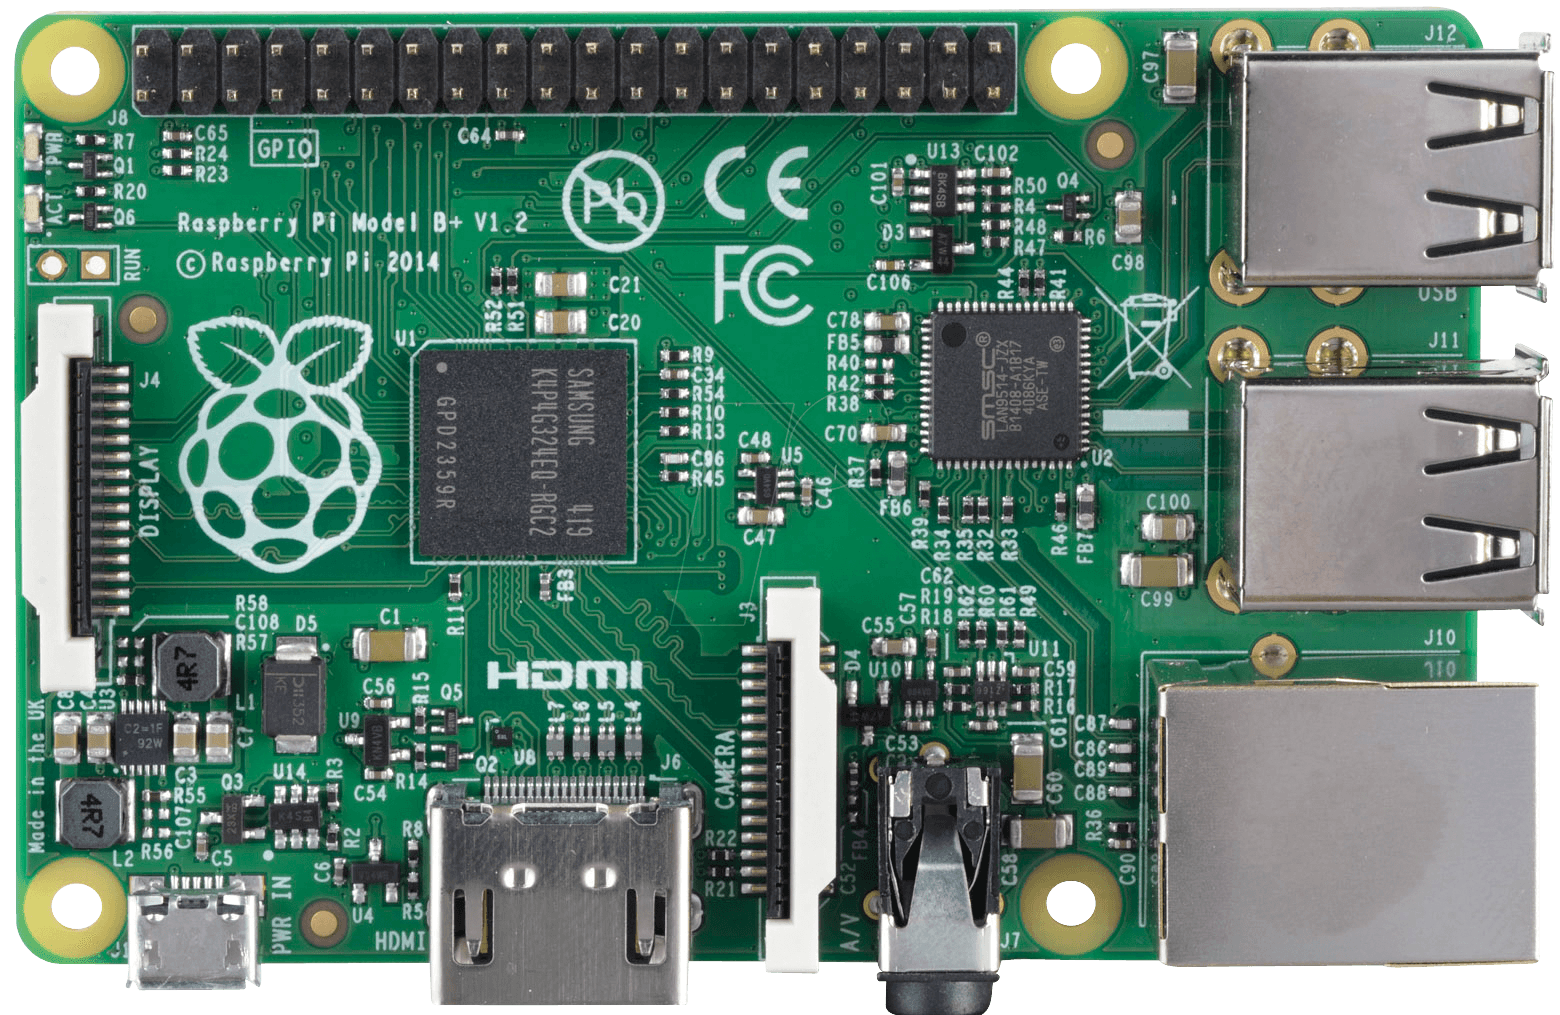
\includegraphics[width=1\linewidth]{Graphics/raspi24.png}
        \caption{Raspberry Pi 4B}
        \label{fig:enter-label}
    \end{figure}
  
  \subsection{Webcam}
  Webcam is a video camera typically connected to computer or other devices through a USB port. Webcam is used in our project to capture the robot's environment, which is essential for task like object manipulation using robotic arm. 
    \begin{figure}[h]
    \centering
    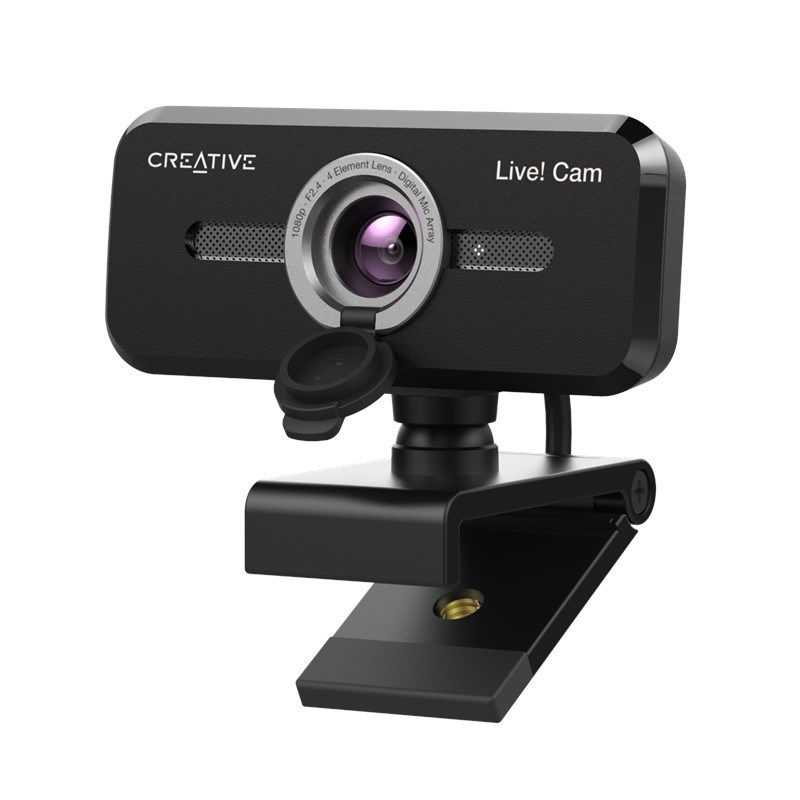
\includegraphics[width=1\linewidth]{Graphics/webcam.jpg}
    \caption{Web Cam}
    \label{fig:enter-label}
\end{figure}
  
  \subsection{MG996r Servo Motor}
  MG996r is a popular servo motor commonly used in robotics project. It is known for its high torque output, making it suitable for applications that require strong and precise movements.
  \begin{figure}[h]
    \centering
    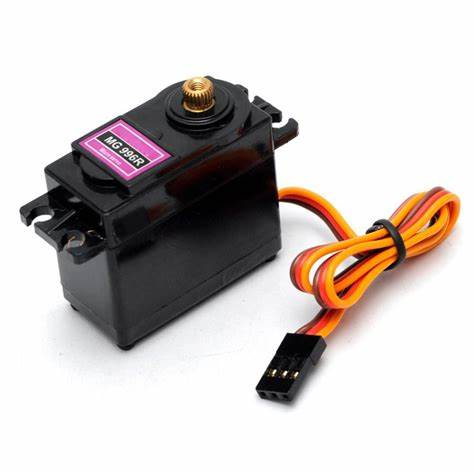
\includegraphics[width=1\linewidth]{Graphics/servoooo.jpg}
    \caption{Servo mg996R}
    \label{fig:enter-label}
\end{figure}
  \subsection{MG90s Servo Motor}
  MG90s Servo Motor is popularly known for its compact size and versatility.
  MG90s is a micro sized analog servo motor. Due to its compact size it is convenient to accommodate in small robotic projects.
  \subsection{16-Channel Servo Controller}
  A 16-channel servo controller is a device designed to control up to 16 servo motors simultaneously. Since we are using two servo motors in our project, it ensures precise control of both the servo motors.
  \subsection{Buck Converter}
  A buck converter, also known as a step-down converter, is a type of DC-DC power converter that transforms a higher voltage level into a lower one. It is able to regulate the output voltage despite the variations in the input voltage.
  \begin{figure}[h]
    \centering
    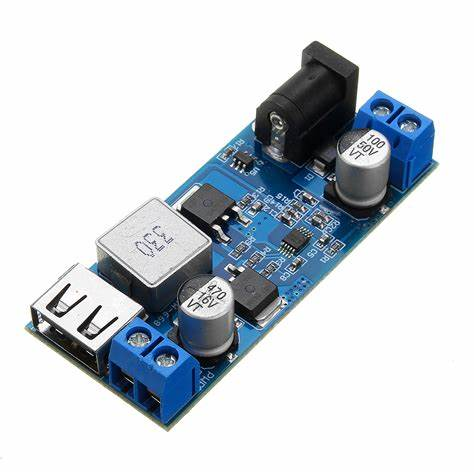
\includegraphics[width=1\linewidth]{Graphics/buckconverter.jpeg}
    \caption{Buck Converter}
    \label{fig:enter-label}
\end{figure}
\subsection{Ultrasonic Sensor}
An ultrasonic sensor works by emitting high-frequency sound waves (ultrasonic waves) and measuring the time it takes for the waves to bounce back after hitting an object. It consists of a transmitter that sends out ultrasonic pulses and a receiver that detects the echoes. By calculating the time difference between sending the signal and receiving the echo, the sensor can determine the distance to the object based on the speed of sound in the medium. Typically, ultrasonic sensors operate in the range of 20 kHz to 200 kHz, with higher frequencies providing better resolution but shorter range. They are commonly used in robotics, distance measurement, and object detection applications due to their accuracy, reliability, and non-contact nature.
\begin{figure}[h]
    \centering
    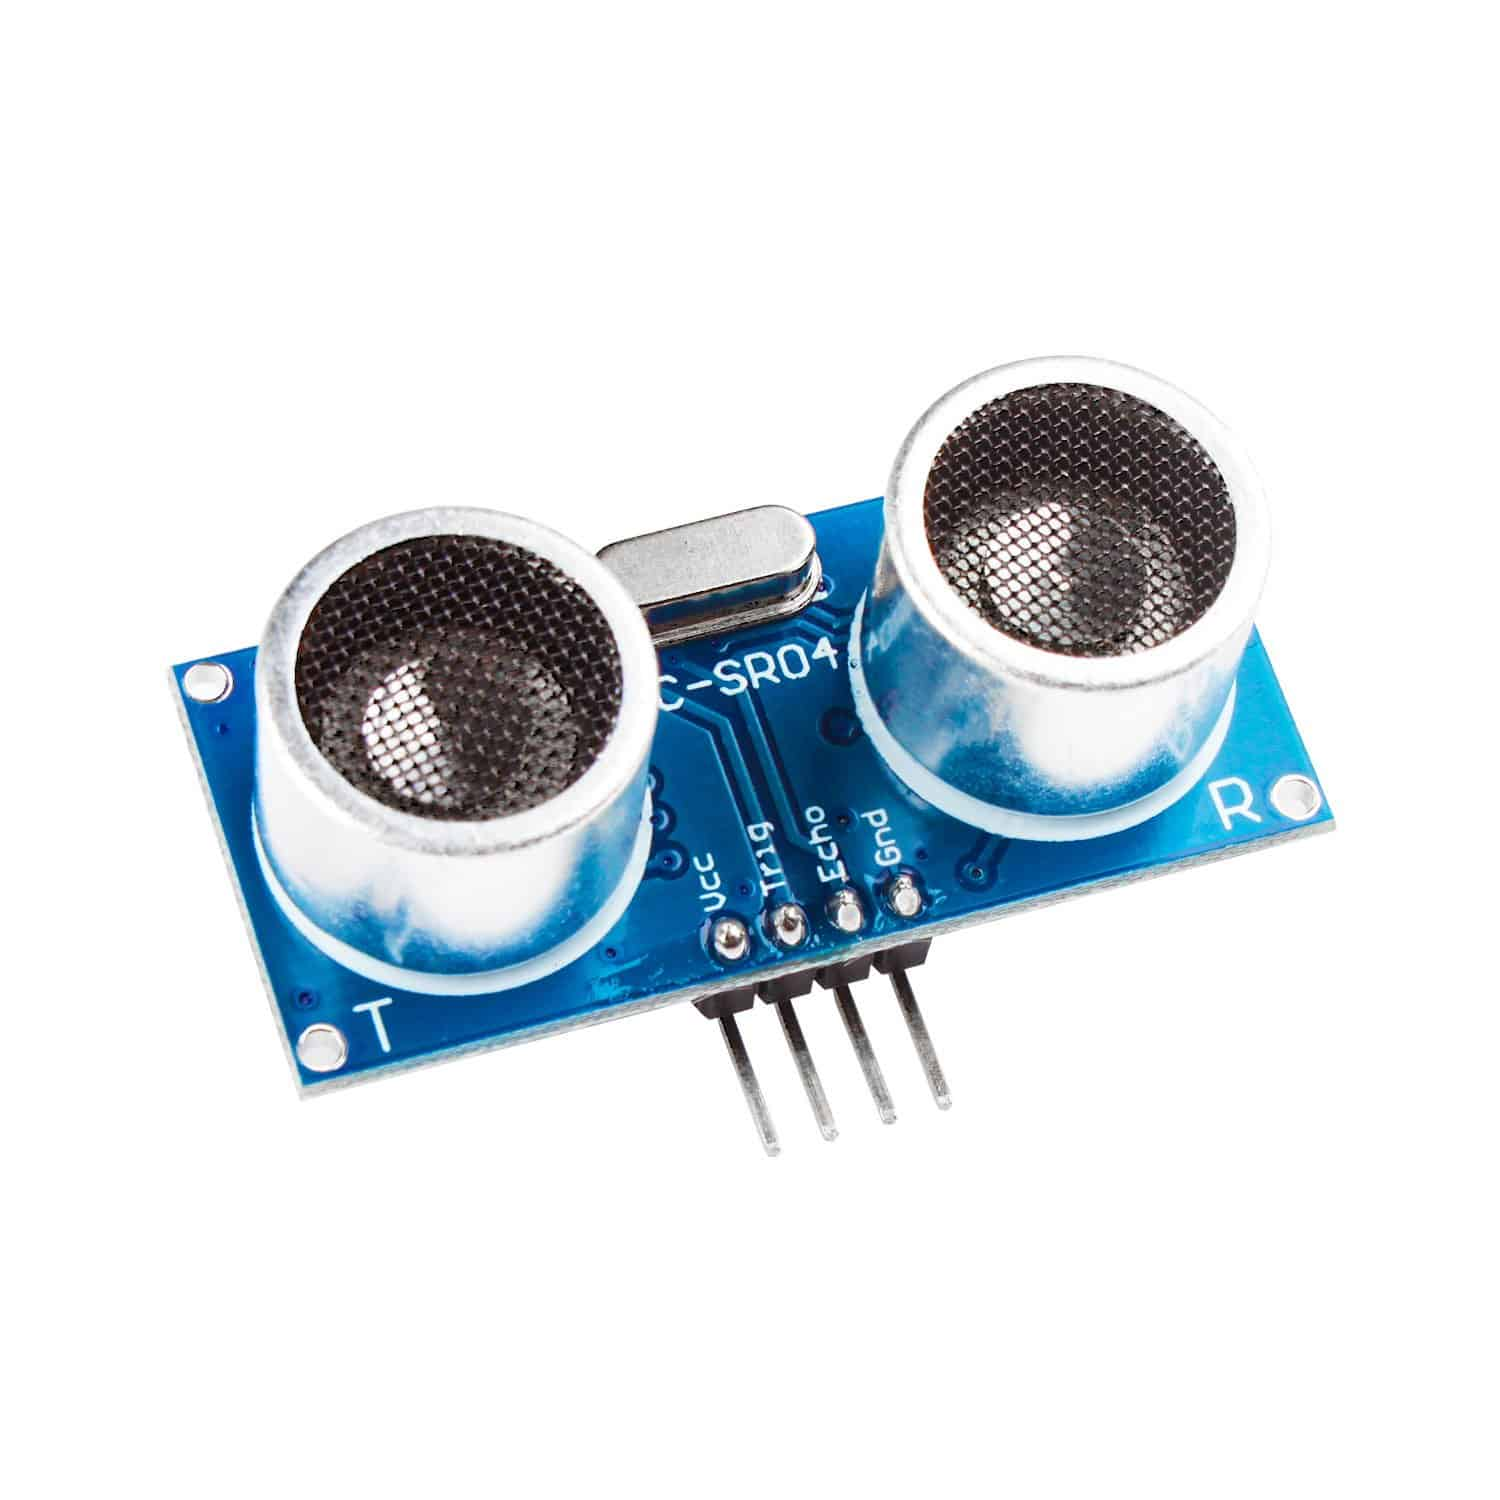
\includegraphics[width=1\linewidth]{Graphics/ultrasonicSensorImg.jpg}
    \caption{Ultrasonic Sensor}
    \label{fig:enter-label}
\end{figure}

  \section{Software Requirements}
\subsection{Python}
Python is a general-purpose language suitable for a wide range of applications, including web development, data science, artificial intelligence, automation, scientific computing, and more. Python library, SpeechRecognition was utilized to capture and interpret voice commands. Similarly, to control robotic arm and motors, to process visual data and so on Python was used in this project.
\subsection{Raspberry Pi OS(Raspbian)}
It is the official operating system designed for the Raspberry Pi single-board computers. Python is pre-installed and well-supported, making it easy for users to get started with programming on the Raspberry Pi.
\subsection{VNC Viewer}
VNC Viewer is the client application used to connect to a VNC server, enabling you to access and control the desktop of a remote system. VNC Viewer controls and access a Raspberry Pi from a desktop, laptop or mobile devices.
\subsection{VS code}
Visual Studio Code (VS Code) is a lightweight yet powerful source code editor developed by Microsoft. It offers a wide range of features tailored for software development, including syntax highlighting, code completion, debugging support, version control integration, and extensibility through a vast ecosystem of extensions. VS Code is built on the Electron framework and runs on Windows, macOS, and Linux. Its user-friendly interface, coupled with robust customization options and built-in terminal support, makes it a popular choice among developers across various programming languages and platforms. Additionally, VS Code's IntelliSense feature provides intelligent code suggestions, helping developers write code faster and with fewer errors. Overall, VS Code's versatility, performance.

\chapter{LITERATURE REVIEW}
A robot may define as an electro-mechanical device, which
is capable of sensing its surrounding and taking its decision
(command).In general, robot must be able to move (by
mechanical movement), it must be able to sense (by
transducer) and it should be take decision (by remote
control or artificial intelligence). A robotic arm is a robot
manipulator, which can perform similar functions to a
human arm.
Robotics arm is vital role of industrial application. Most
robotics arm perform the task such as welding, trimming,
picking, placing and painting etc \cite{r1}.

Some    basic    applications    of    robots    utilizing    voice recognition  are  to  support  elderly  people  or  people  with disability,  voice  controlled  personal  assistance  etc . The   Raspberry   pi   board   has   several   applications,   from distance measurement of a target object from another object for  the  purpose  of  civil  engineering  to  developing  a robotic arm to help medical staff and elderly people. Instead of   using   multiple   dynamic   interfaces,it   is   easier   to communicate with machines through voice commands\cite{r2}.

Raspberry Pi is a series of small single-board computers developed  in  the  United  Kingdom  by  the  Raspberry  Pi Foundation in association with Broadcom. The Raspberry Pi is   a   lightweight,   powerful,   inexpensive,   hackable,   and educational  computer board  .  The  Raspberry  Pi was  introduced  in  2012,  and  several  versions  and  variants have  since  been  released.  The  original  Raspberry  Pi  had  a single-core  700MHz  CPU  and  just  256MB  RAM,  and  a quad-core 1.4GHz CPU with 1GB RAM is available for the new  edition.  For  Raspberry  Pi,  the  main  price  point  has always  been  \$ 35,and  all  models  have  been  \$35  or  less, including the Pi Zero, which is just \$5 .Some of these  devices  are  necessary,  others  are  optional,  but  all Raspberry Pi models have the same BCM2835 CPU, which is  inexpensive,  efficient,  and  does  not  consume  a  lot  of energy. The Raspberry Pi also utilizes an operating system like any other computer. In  order  to  learn  programming  skills,  create  hardware projects,   do   home   automation   and   even   use   them   in industrial   applications,   people   all   over   the   world   use Raspberry   Pi.   There   have   been   three   generations   of Raspberry  Pi`s:  Pi  1,  Pi  2,  and  Pi  3,  and  most  generations have  usually had a  Model  A and a  Model  B. Model  A  is a cheaper version which appears to have lower RAM and USB and  Ethernet  ports.  The  Pi  Zero  is  a  spinoff,  made  much smallerand cheaper, of the original (Pi 1) generation. Table I provides a comparison of the scale, weight, and cost of the standard Raspberry Pi generation\cite{r2}.

Computer  vision  and  artificial  intelligence  have  been successfully  utilized  to  operate  complex  robotic  systems  in many  works. For instance, in a recent work , the authors designed  an  automatedrobotic  arm-based  assistance deviceby employingsimple   stereo   matching   and   q-learning optimization  techniques.  The  proposed  device  can  perform five degrees of operation in a single instance and detect any object with the help of stereo vision. The system also keeps track  of  an  object's  parameters.  The  stereo  camera  can identify   the   RGB   color.   In   this   work,   the   Q-learningframework is  employed  to  control  the  position  of  the robot’s   arm.   Finally,   the   paper   showed   experiments   to identify  an  object's  stereo  vision  and  feature  point.  The downfall  of  the  study  is  that  it  did  not  specify  the  exact distance between the objects \cite{r3}.

Both the purpose of optimizing today's industrial production and integrating various
technologies is the goal of Industry 4.0. Thus, it is critically important issue to integrate the
information system with the information in the real space through the Internet, such as, the
IoT (Internet of Things), big data, AI (artificial intelligence) and other diverse customized
manufacturing. A single-function target is adopted in traditional industrial manufacturing with
most of the mechanical arms. The advantage of combine with integrated system of complete
work is that they can complete quick and accurately to pick an objects and to move to a
suitable place at the same time. Such behavior can reduce the time for complicating the
operations convenience, and also totally improve the allocation of human resources .
However, under the influence of globalization in order to apply those substantial monitoring
records from the process of production, to make more advanced technical planning with the
assistance of high technique is necessary. The consideration to apply an auxiliary tool that can
bring huge profits to the enterprise, apply precise robotic arms maximizes the usage of all
machine equipments in the factory, and even to monitor the signal for handling the production
of components in the factory are some most strategies carried out in a factor. Especially, if an
enterprise is trying to transform the flow of manufacturing. Record and report timely to
information are importantly required, such as storage, storage location, management
personnel, etc., and effectively predict the loss of the machine, fault maintenance, and even
reduce operating costs caused by misjudgment. Moreover, how to embed human thinking and
behavior capabilities into a robots let it becomes smarter, more agile, and even low-cost,
which is worth thinking. It is possible to establish a new model of cooperation between the
human and machine. Under the cooperation of man and machine, robots can not only help
humans complete cumbersome and dangerous special tasks, but also transmit the lowest-level
information .\cite{r4}.

In today’s world, time and man power are important constraints for the completion of tasks. Robots are used in
industries to perform simple repetitive tasks. Compared to humans, robots complete tasks faster and with greater accuracy.
They are increasingly used in industries to automate tasks in an assembly line for pick and place. Robot arms are used as a
pick and place robot in industries. This paper presents a robot arm used as a pick and place robot using a raspberry pi
microcontroller. The robot arm can automatically move to a location where the object to be lifted and placed. Ultrasonic
distance sensors are installed at the robot arm to recognize the object. The robot arm is used to hold the object and move it to
desired destination.\cite{r5}
\chapter{METHODOLOGY}
\section{Overview}
The project we are developing combines the power of voice recognition and computer vision to create a highly advanced and intuitive robotic system. Our robot is programmed in such a way that it recognizes the commands given by the operator, understands it and performs the specified operation which can be termed as human-robot interaction.

\section{Data Collection}
For the succession of our project, research and data collection played a major part. The methods used for collecting data required for our project included observations and secondary data analysis. By observing and experimenting the process we selected the suitable method. Similarly, all the documents and records available in the internet guided us throughout this project.
\section{Tools and Technologies}
\subsection{Hardware}
The project's hardware consists of a central control unit such as a Raspberry Pi. It also includes a robotic arm kit, an ultrasonic sensor for measuring distance, a camera module for computer vision tasks, motors, motor drivers, and peripheral like a microphone for voice interaction. These hardware components create the physical structure of the voice-controlled robot, enabling its mobility, sensing, and interaction with the surroundings.
\subsection{Software}
Python is the main programming language used for implementing the robot's functions in the project. OpenCV is utilized for computer vision tasks to help the robot understand its environment. TensorFlow is used to train the object detection model, which enables the robot to recognize and locate objects. Speech recognition libraries are incorporated to process voice commands for controlling the robot. Motor control libraries are also used to ensure precise movement of the robot, allowing it to perform tasks accurately. These software elements are essential for integrating voice control, computer vision, and robotic arm functions seamlessly within the robot system.
\section{System Block Diagram}
\begin{figure}[h]
    \centering
    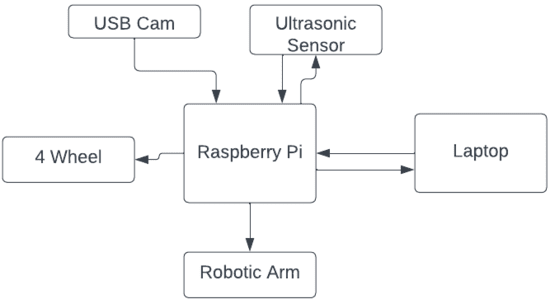
\includegraphics[width=1\linewidth]{systemBlockDiagram (1) (1).png}
    \caption{Voice Controlled Robot System Block Diagram}
    \label{fig:enter-label}
\end{figure}

\newpage
\section{System Flowchart}
\begin{figure}[h]
    \centering
    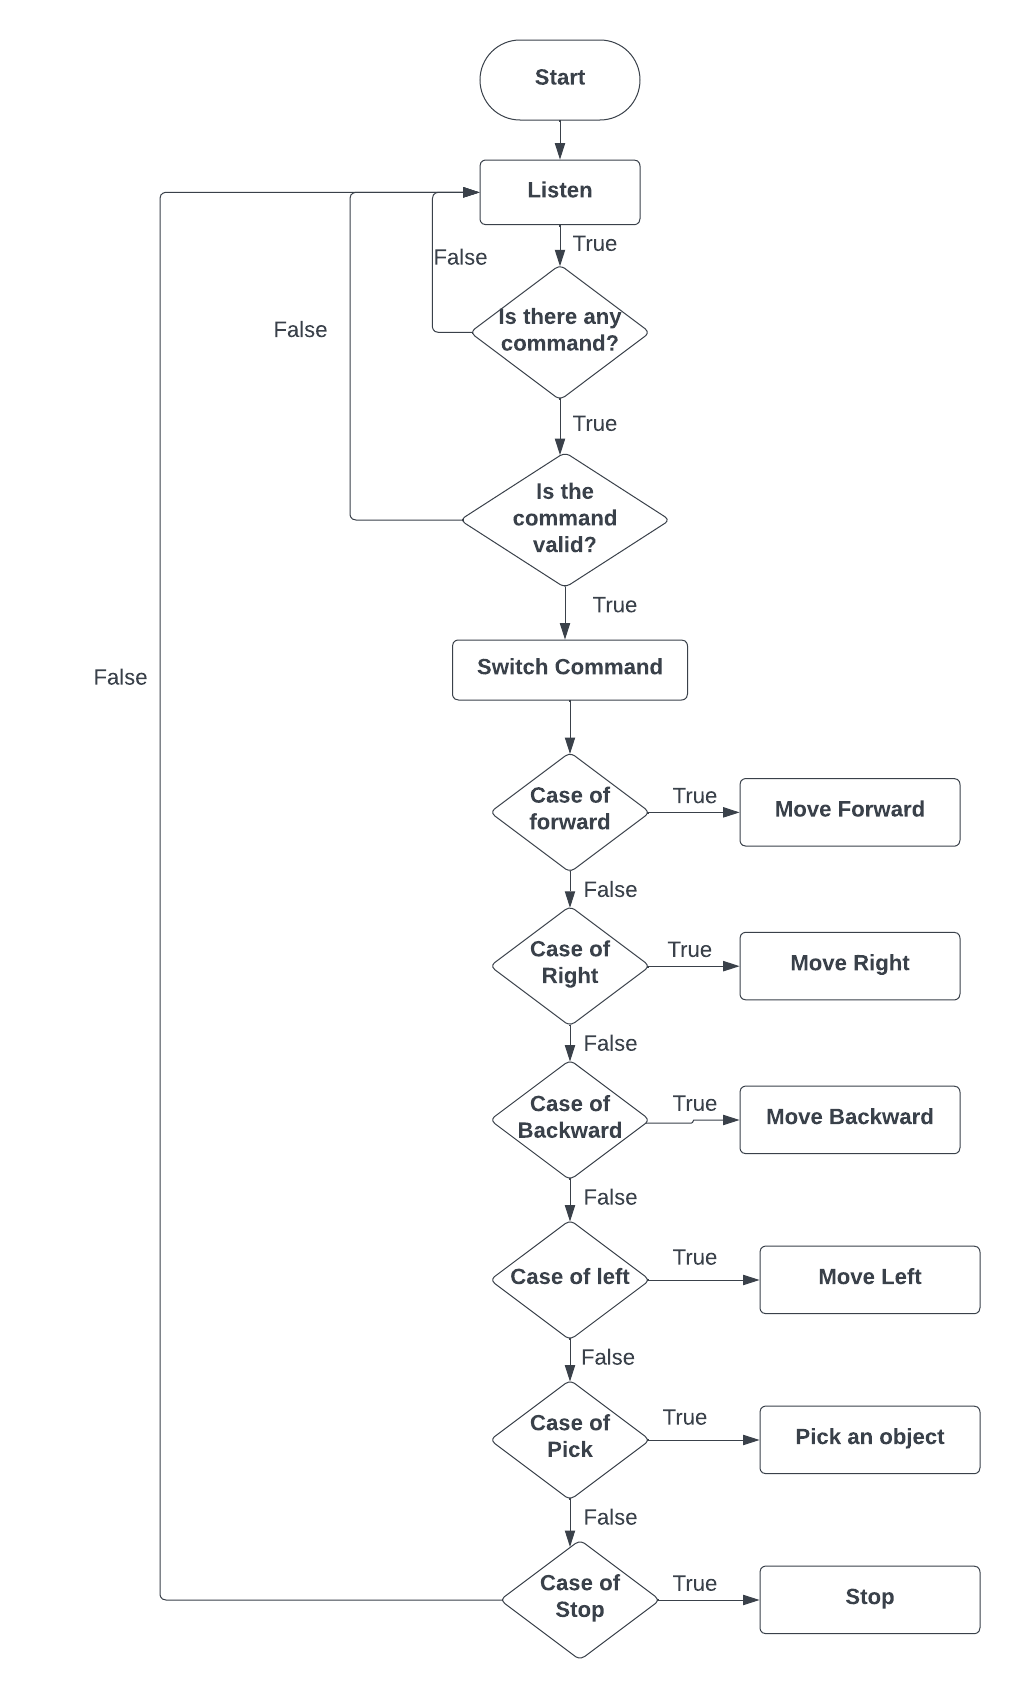
\includegraphics[width=0.7\linewidth]{systemFlowchart.png}
    \caption{System Flowchart}
    \label{fig:enter-label}
\end{figure}
\newpage
\section{Working Principle}
Our project is based on voice control and general AI robotics. The prime idea is to give 
commands to our robot and expect its performance accordingly. Our robot is 
programmed in such a way that it recognizes the commands given by the operator, 
understands it and performs the operation as specified by the operator. The operations 
can be vivid like: following the operator, moving in any direction as specified, picking 
various objects, etc. All-of these operations can be done with the help of computer 
vision, speech recognition, ML and a micro-controller like: Arduino. Although various 
other operations can be programmed, in our project we have programmed a few 
operations that will be seen in the robot's operations.
\section{Limitations}
\begin{itemize}
    \item \textbf{Speech Recognition Accuracy:} Voice recognition systems may not always 
accurately understand spoken commands, especially in noisy environments or with 
accents or speech variations. This can lead to misinterpretations and unintended 
actions by the robot.
    \item \textbf{Limited Vocabulary:}Training the speech recognition system to understand a vast 
vocabulary can be challenging. A limited set of recognized commands might 
restrict the robot's versatility and interactions with users. 
    \item \textbf{ Processing Time:}Real-time voice recognition and image processing can be 
computationally intensive, particularly on low-power microcontroller like those 
commonly used in robotics. This may lead to delays in response time and affect 
the robot's overall performance.
    \item \textbf{Recognition Complexity:}Object recognition algorithms may struggle with certain 
objects or in varying lighting conditions, leading to inaccurate or failed detection.
\end{itemize}

\include{Resultsanddiscussion}
\chapter{CONCLUSIONS AND FUTURE ENHANCEMENT}
\section{Conclusions}
Through the integration of voice recognition, computer vision, and robotic manipulation technologies, this project enables the creation of a versatile and interactive robotic system capable of performing various tasks and responding to user commands.

In summary, the voice-controlled robot with a computer vision-based robotic arm project serves as a compelling platform for innovation, learning, and exploration in the exciting field of robotics and artificial intelligence. Through creativity, dedication, and a spirit of inquiry, we can unlock new possibilities and shape the future of human-robot interaction.

\section{Future Enhancement}
\begin{itemize}
    \item More sophisticated computer vision algorithms can be implemented to enable identification of wider range of a object.
    \item The size and strength of the robotic arm can be increased for industrial applications.
    \item Natural language processing techniques to enhance the voice recognition capabilities can e integrated. 
    \item Sensors and mapping techniques can be used for the robot to navigate autonomously in its environment. 
    \item More intuitive and natural interfaces for human-robot interaction can be researched and developed.
\end{itemize}


\addcontentsline{toc}{chapter}{REFERENCES}
\renewcommand{\bibname}{\centering REFERENCES}
\bibliographystyle{IEEEtran}
\bibliography{refe}

\addcontentsline{toc}{chapter}{APPENDIX}

\centering{\textbf{APPENDIX A}}
\vspace{1cm}
\begin{figure}[h]
    \centering
    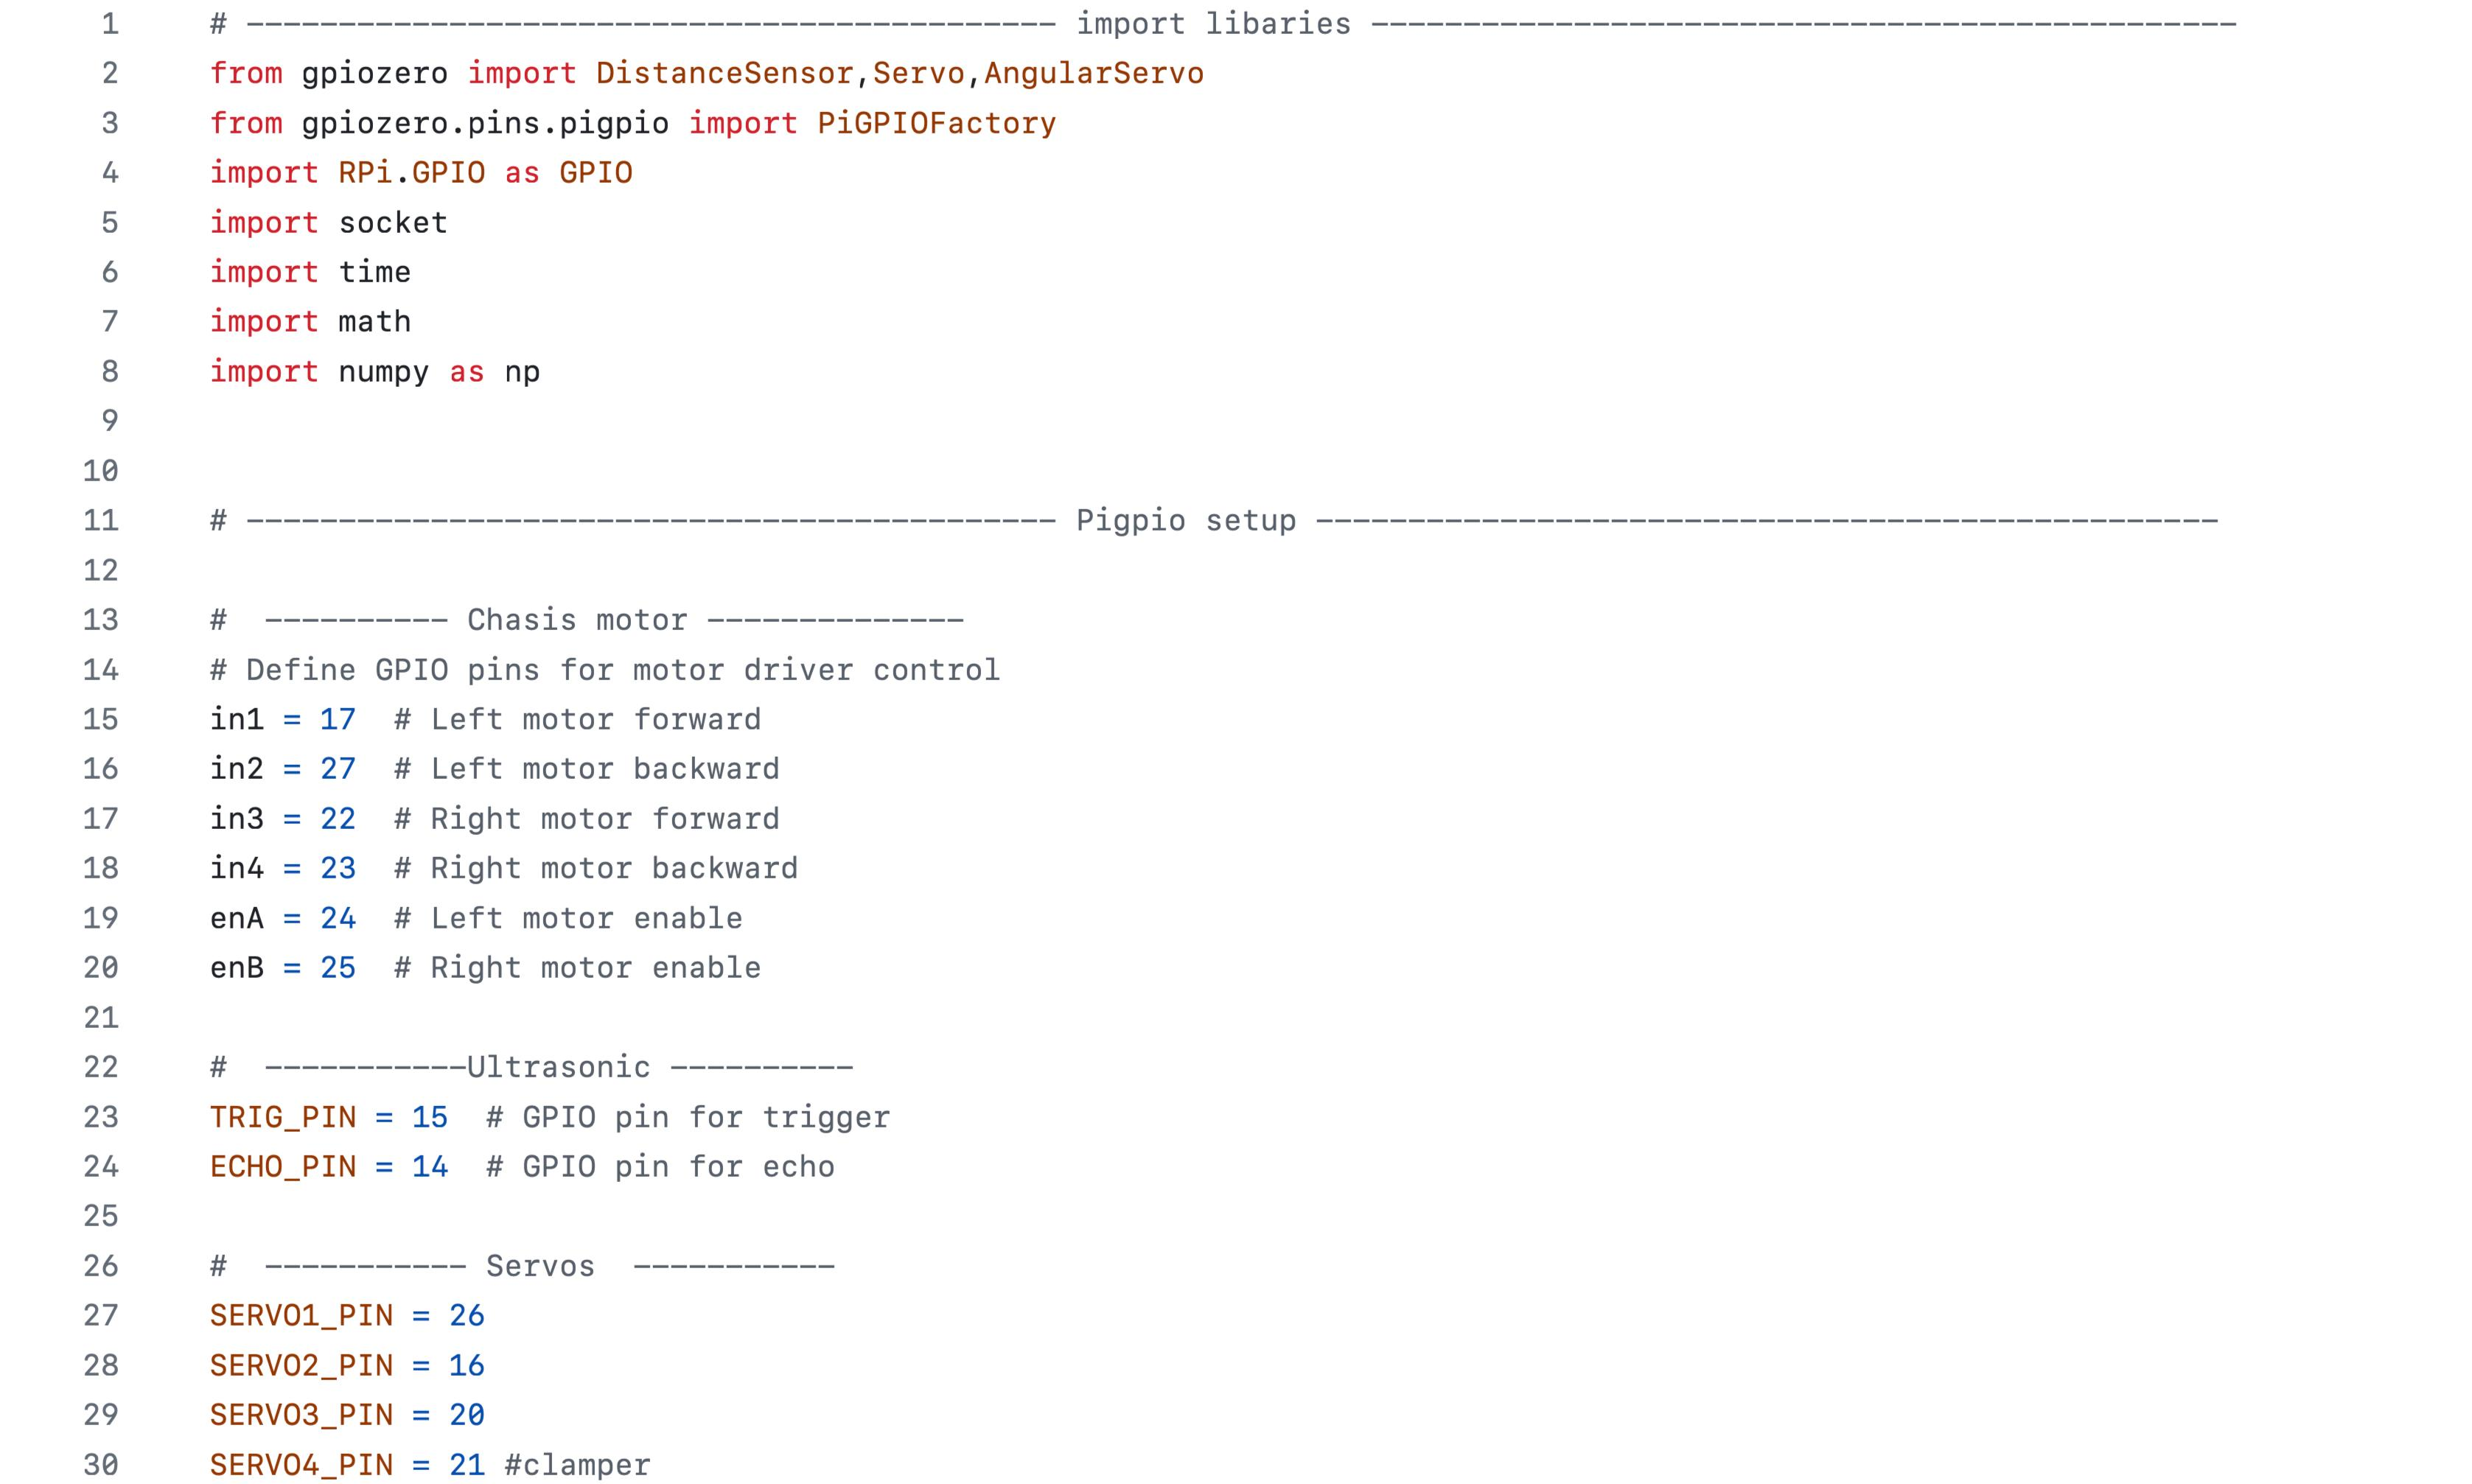
\includegraphics[width=1\linewidth]{Graphics/1pin_assign.jpg}
    \caption{Pin Setup}
    \label{fig:enter-label}
\end{figure}
\begin{figure}[h]
    \centering
    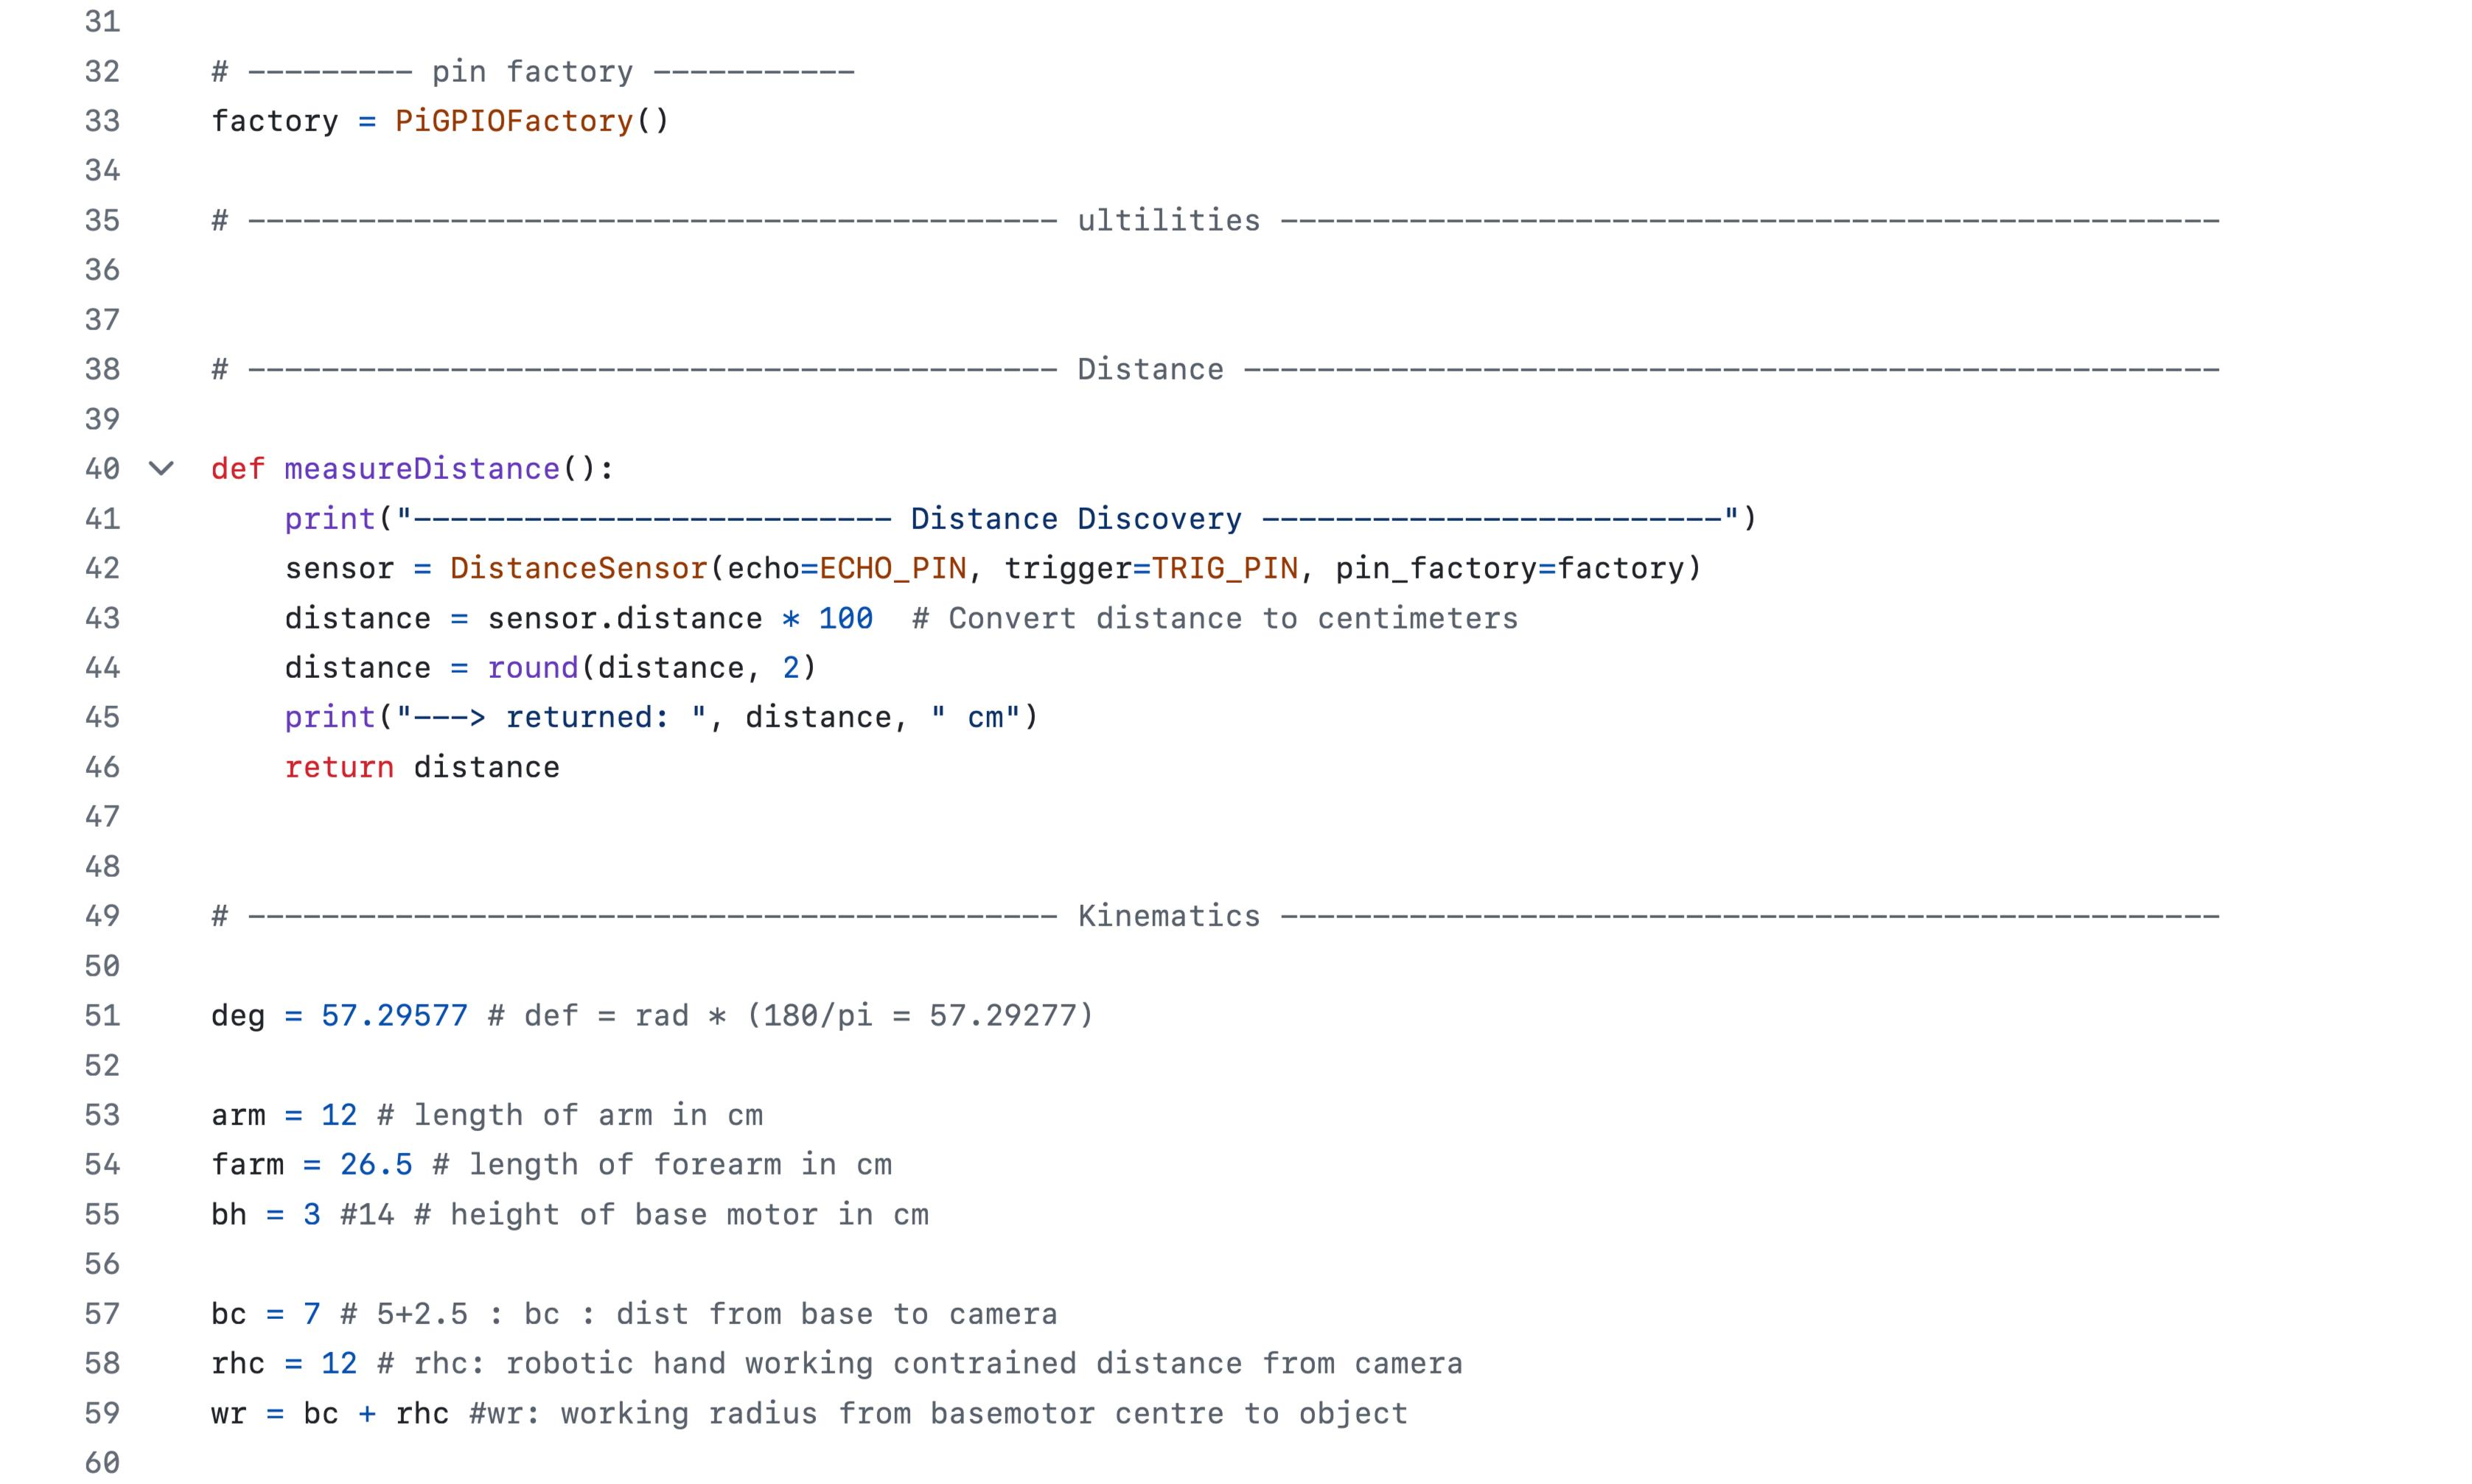
\includegraphics[width=1\linewidth]{Graphics/2distanceMeasurement.jpg}
    \caption{Distance Measurement and Kinematics}
    \label{fig:enter-label}
\end{figure}
\begin{figure}[h]
    \centering
    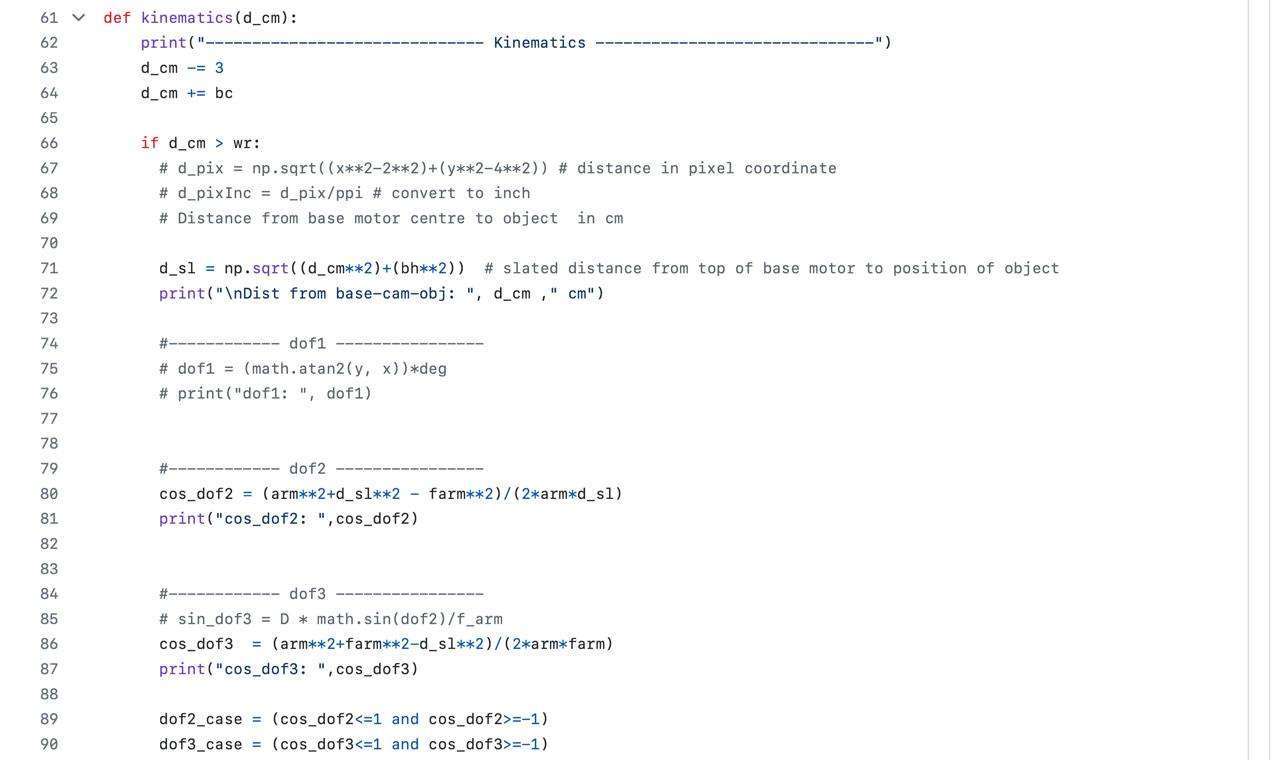
\includegraphics[width=1\linewidth]{Graphics/3kinematics.jpg}
    \caption{Kinematics}
    \label{fig:enter-label}
\end{figure}
\begin{figure}[h]
    \centering
    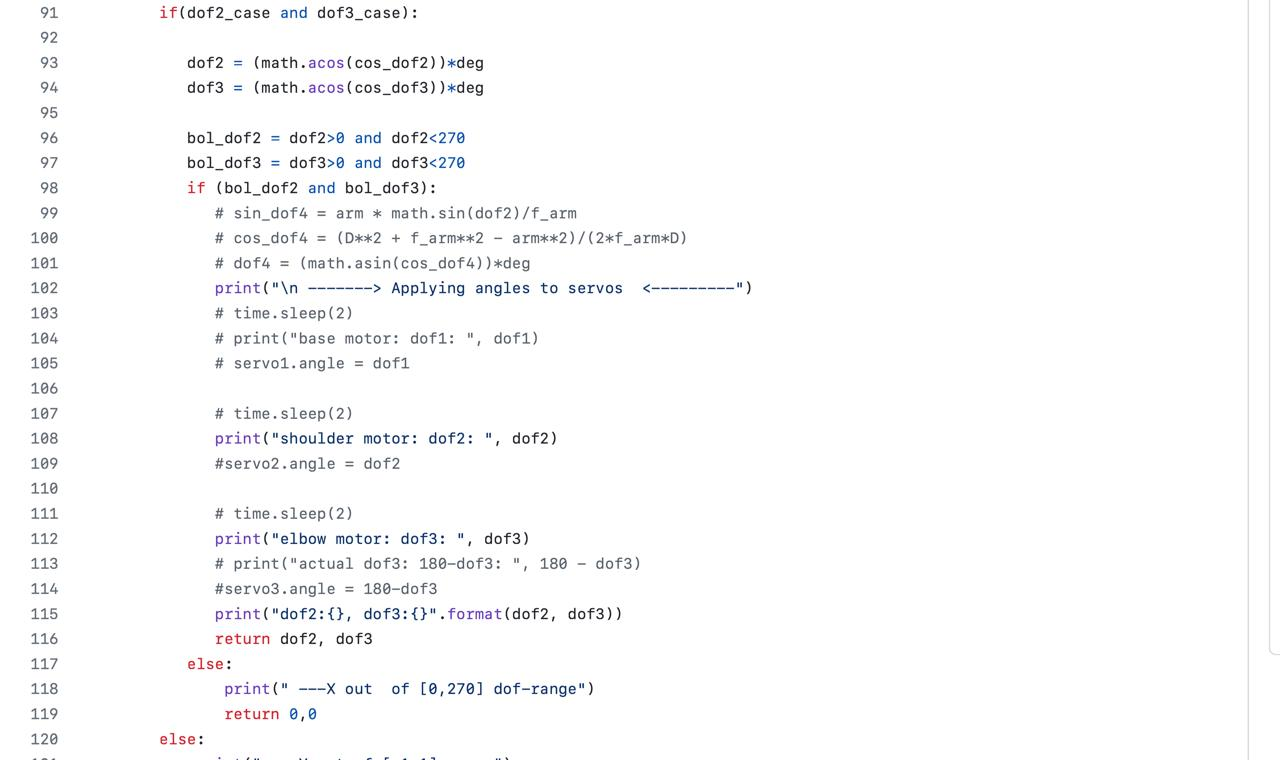
\includegraphics[width=1\linewidth]{Graphics/4anglesToservos.jpg}
    \caption{Angles to Servos}
    \label{fig:enter-label}
\end{figure}
\begin{figure}[h]
    \centering
    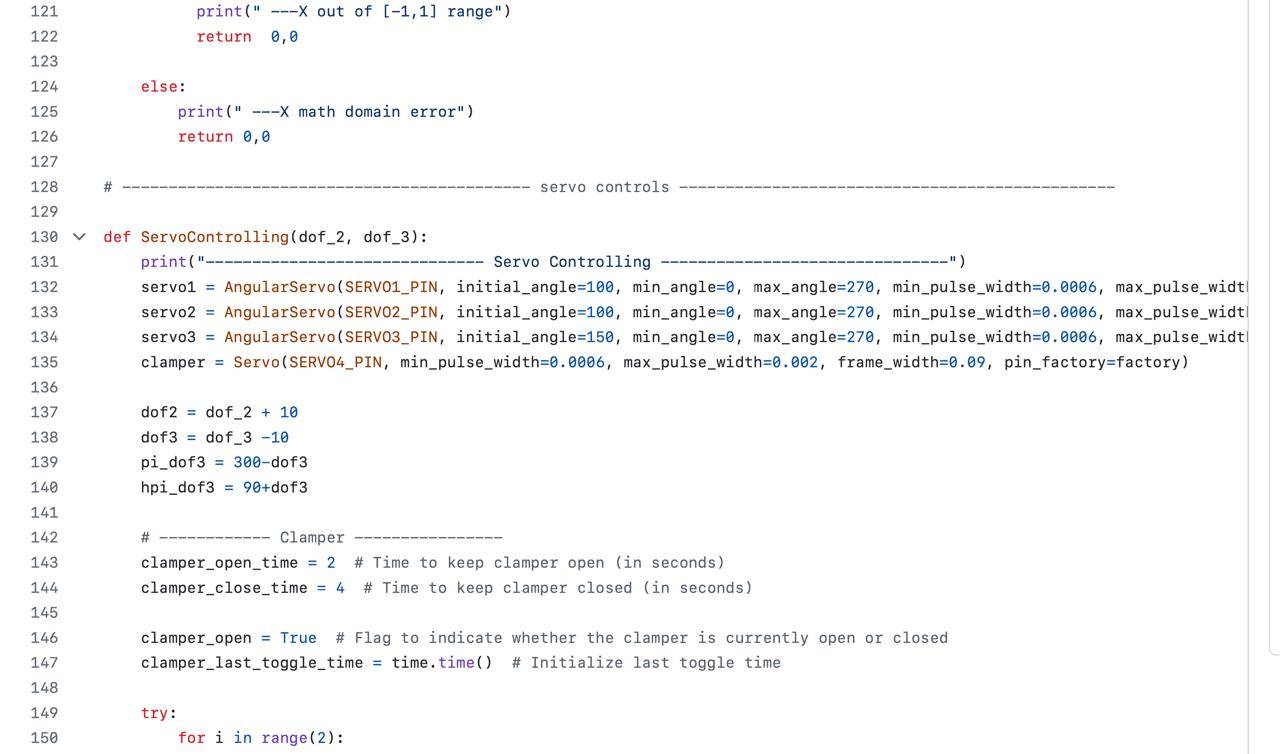
\includegraphics[width=1\linewidth]{Graphics/5servoControl.jpg}
    \caption{Servo Controls}
    \label{fig:enter-label}
\end{figure}
\begin{figure}[h]
    \centering
    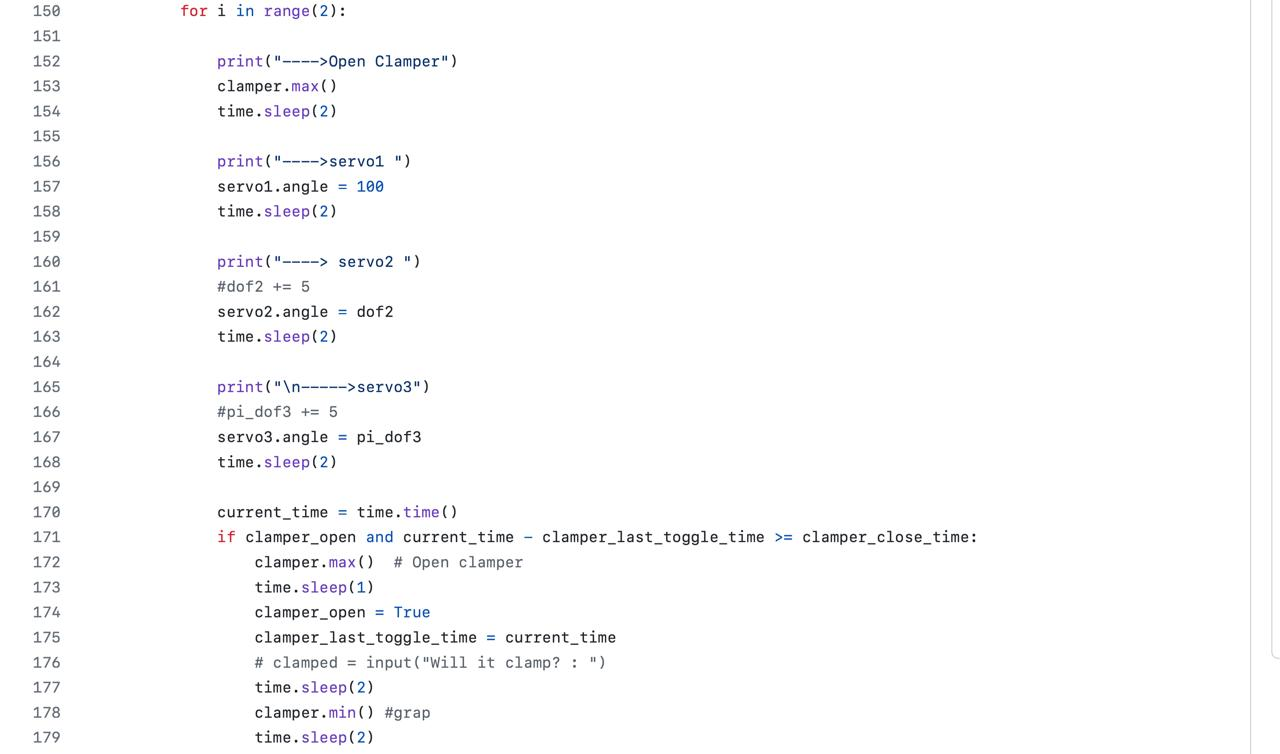
\includegraphics[width=1\linewidth]{Graphics/6clamperOperation.jpg}
    \caption{Clamper Function}
    \label{fig:enter-label}
\end{figure}
\newpage
\vspace{1cm}
\begin{figure}[h]
    \centering
    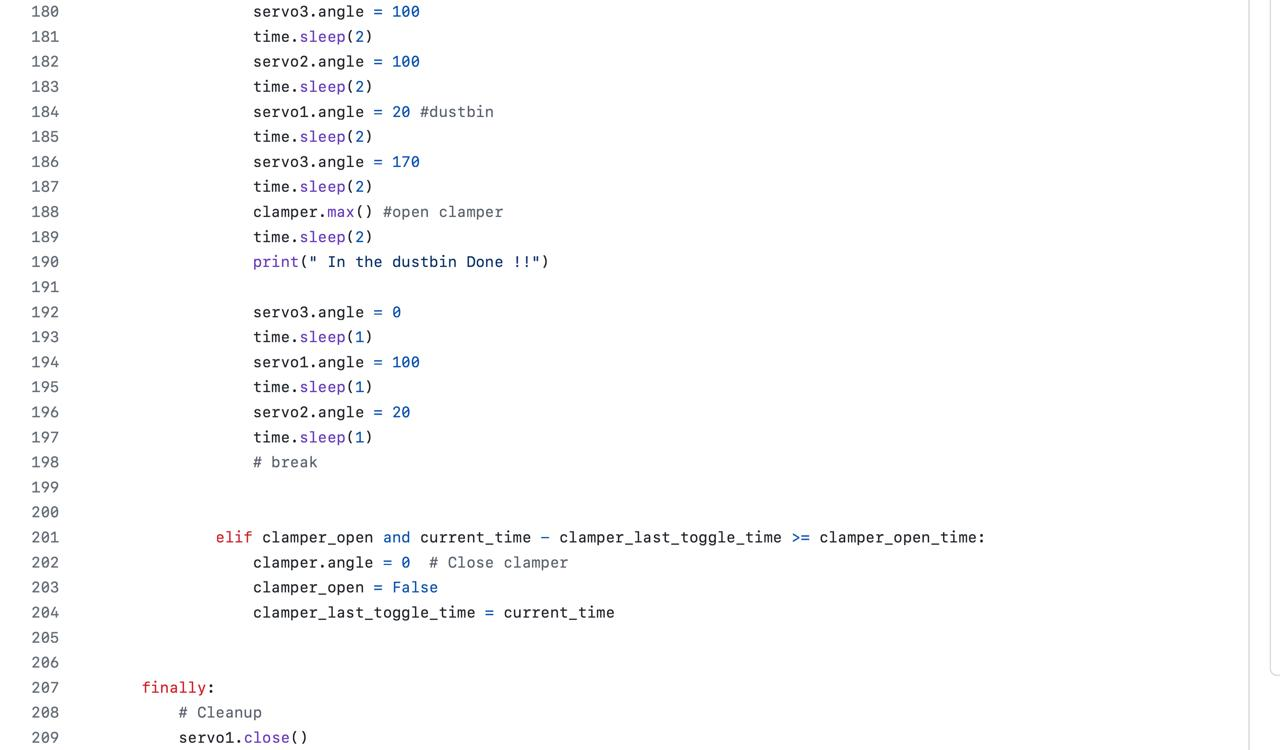
\includegraphics[width=1\linewidth]{Graphics/7clamperWorking.jpg}
    \caption{Clamper Working}
    \label{fig:enter-label}
\end{figure}
\begin{figure}[h]
    \centering
    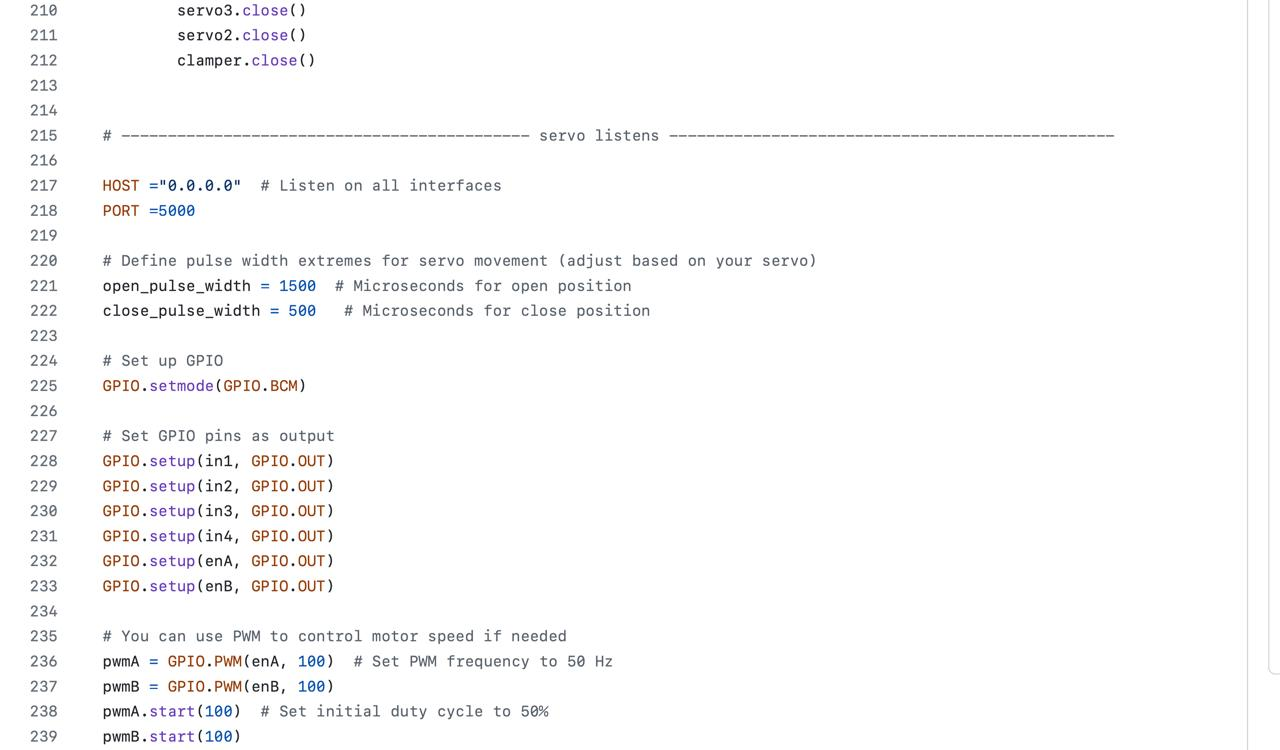
\includegraphics[width=1\linewidth]{Graphics/8ServoInitializing.jpg}
    \caption{Servo Listen}
    \label{fig:enter-label}
\end{figure}
\begin{figure}[h]
    \centering
    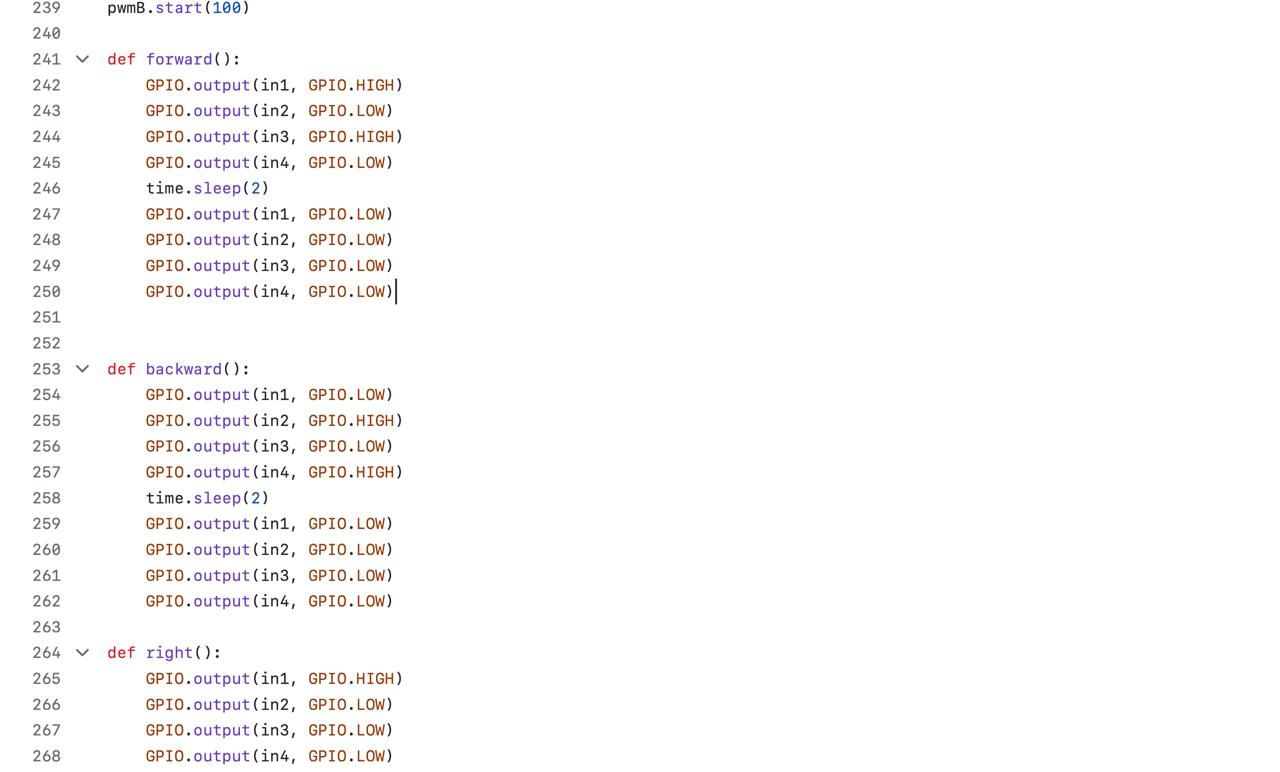
\includegraphics[width=1\linewidth]{Graphics/9functionForBotMotion.jpg}
    \label{fig:enter-label}
\end{figure}
\begin{figure}[h]
    \centering
    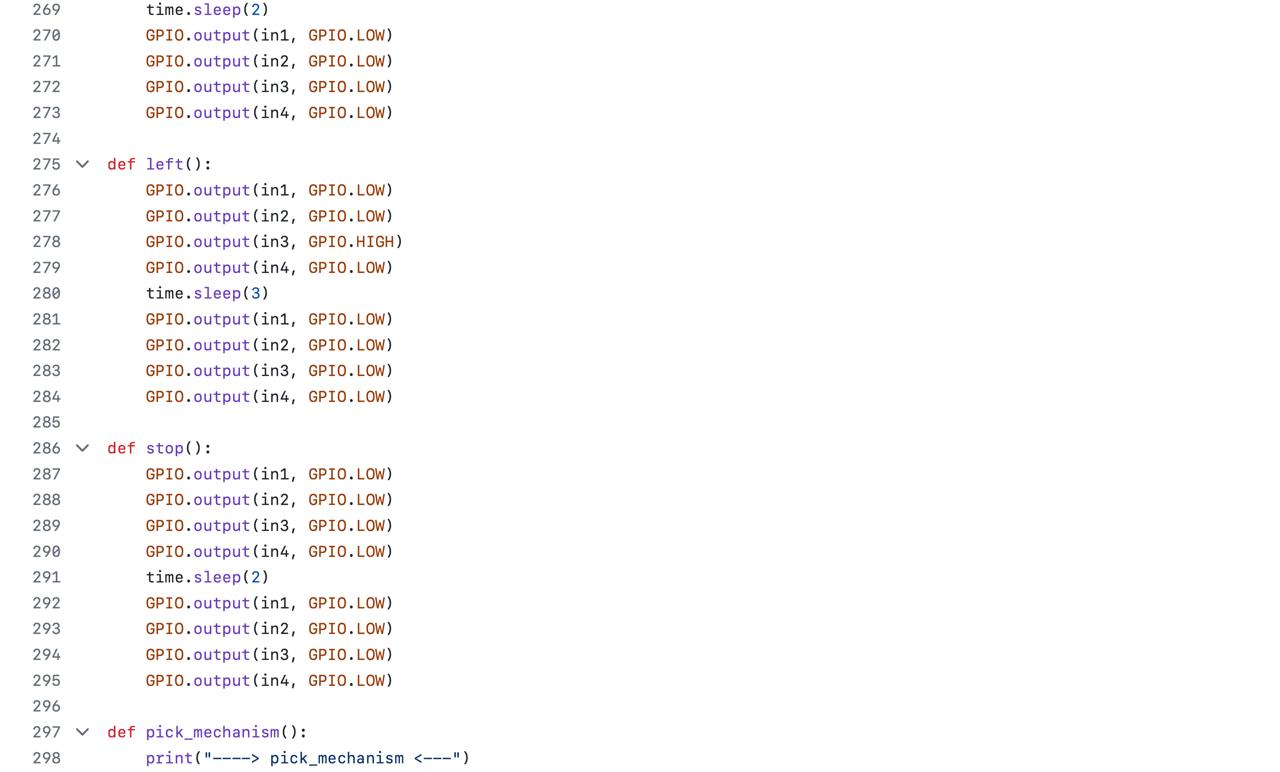
\includegraphics[width=1\linewidth]{Graphics/10 FunctionForBotMotion.jpg}
    \caption{Bot Movement Function}
    \label{fig:enter-label}
\end{figure}
\begin{figure}[h]
    \centering
    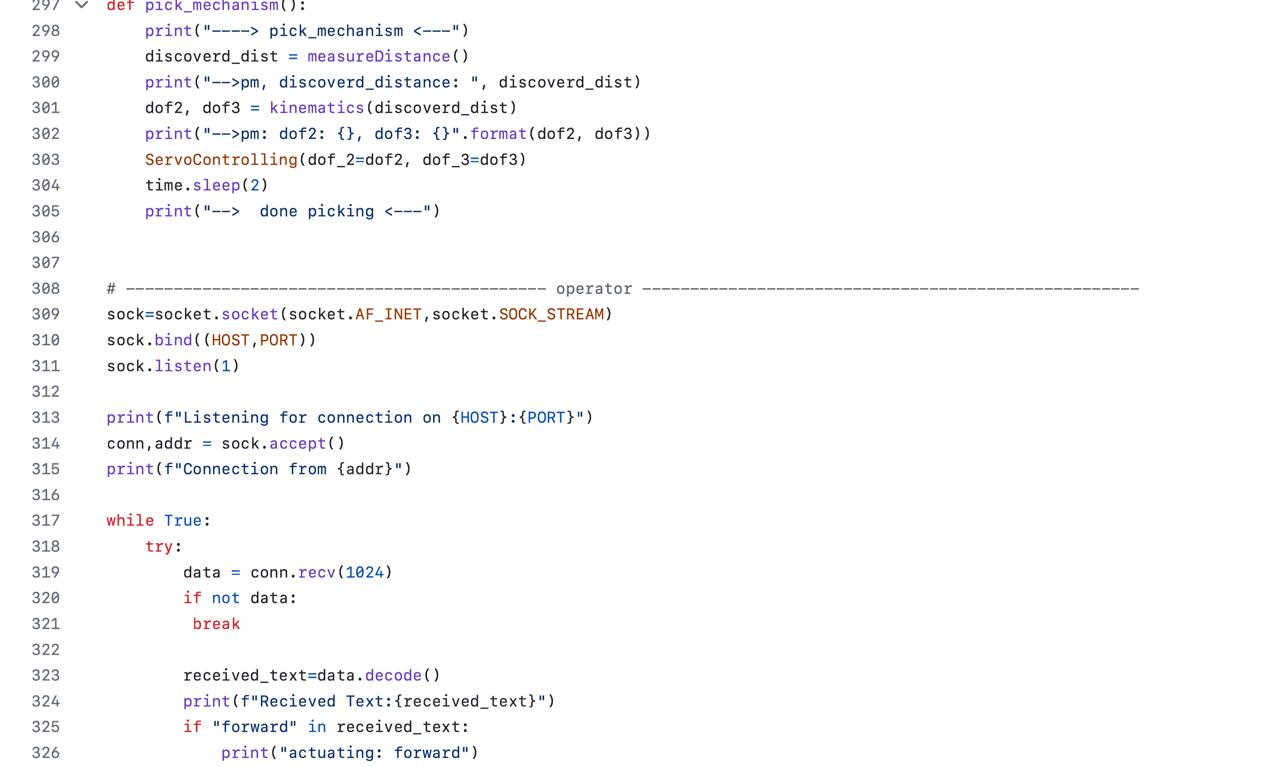
\includegraphics[width=1\linewidth]{Graphics/11functiontoPickAnd socket.jpg}
    \caption{Socket Function to Receive Command}
    \label{fig:enter-label}
\end{figure}
\begin{figure}[h]
    \centering
    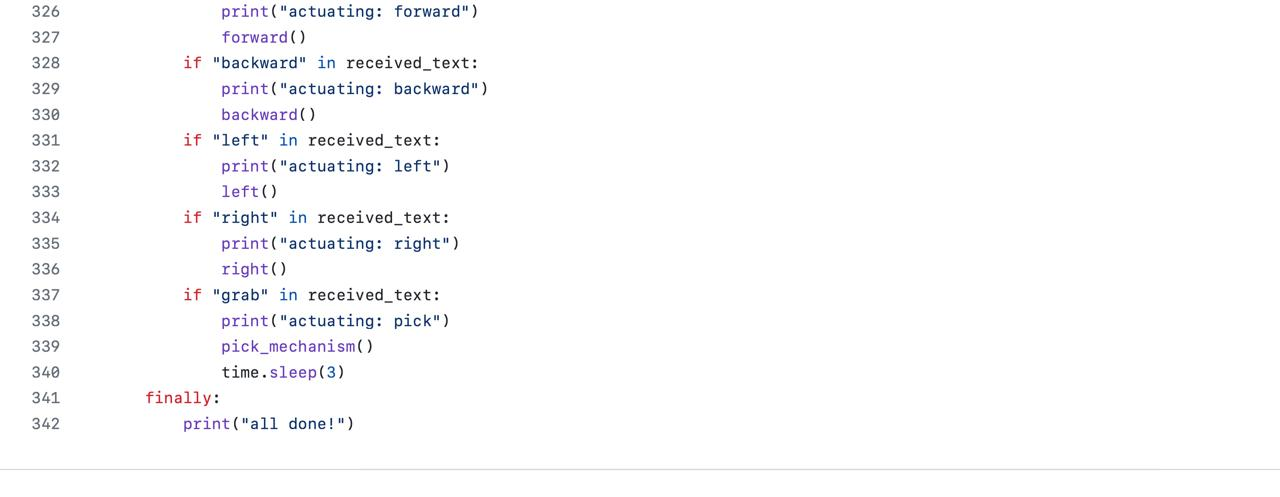
\includegraphics[width=1\linewidth]{Graphics/12voiceCommand.jpg}
    \caption{Voice Command function execution}
    \label{fig:enter-label}
\end{figure}

\begin{figure}[h]
    \centering
    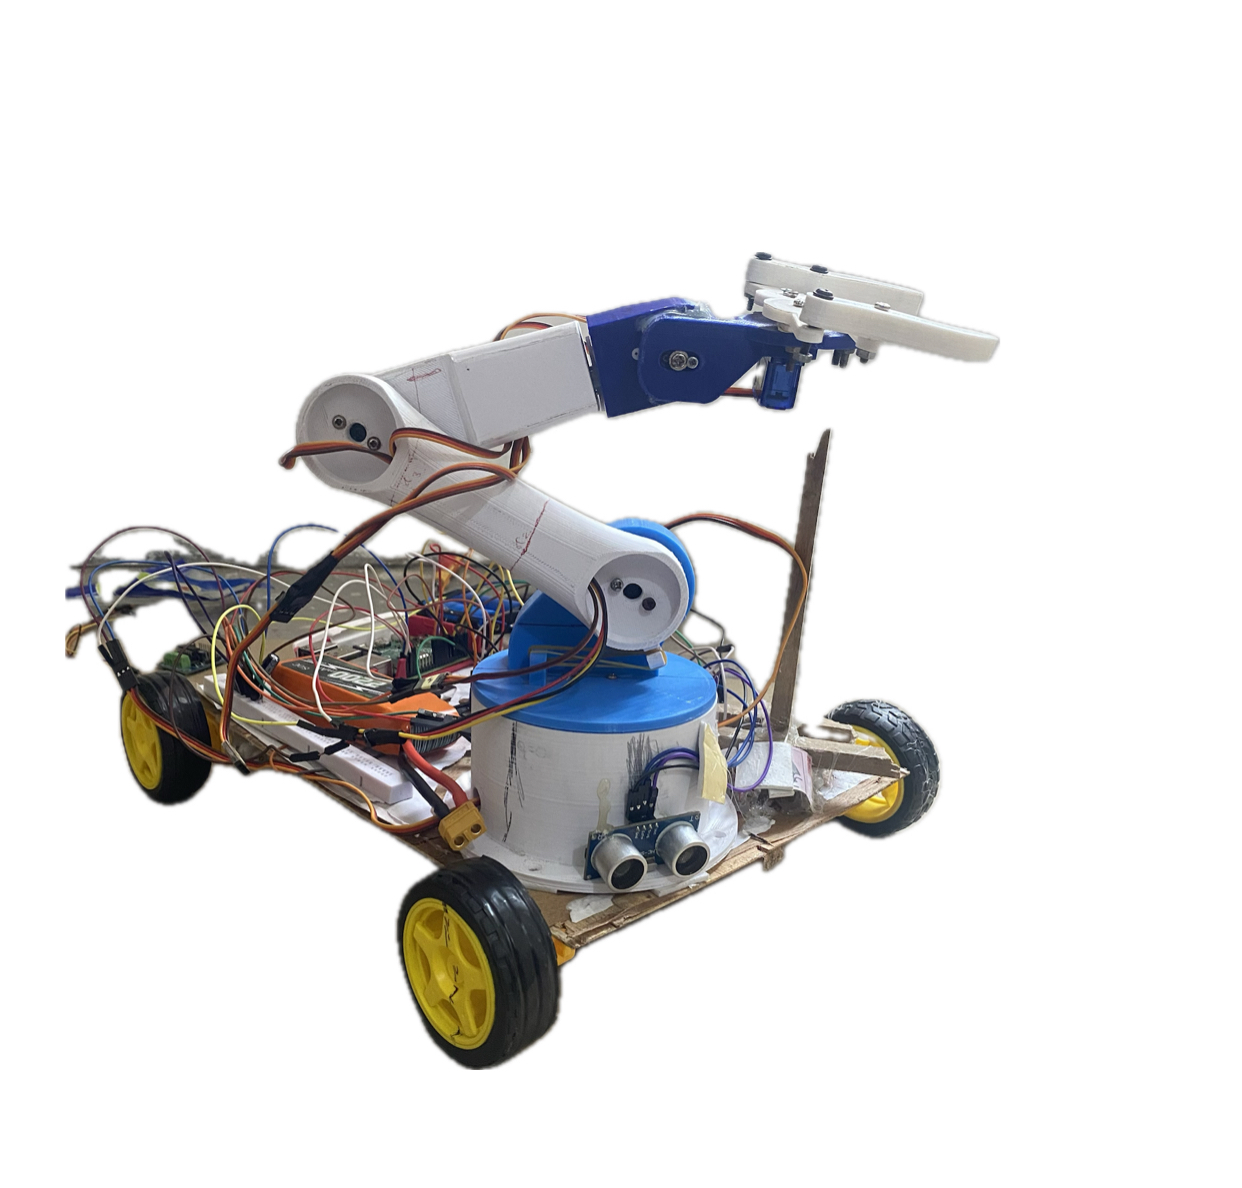
\includegraphics[width=1\linewidth]{Graphics/finalbot.jpg}
    \caption{Bot Model}
    \label{fig:enter-label}
\end{figure}
\addcontentsline{toc}{chapter}{Datasheet}
\begin{figure}[h]
    \centering
    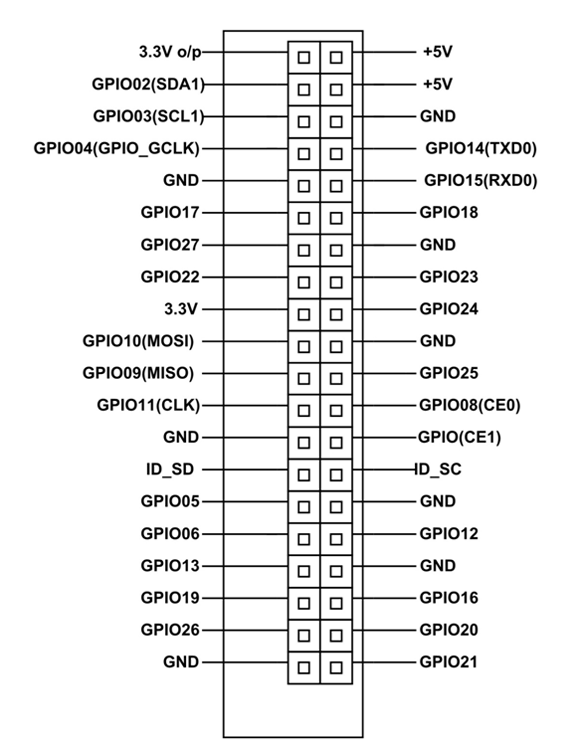
\includegraphics[width=1\linewidth]{Graphics/raspberrypi_pin.png}
    \caption{Raspberry Pi Pin configuration}
    \label{fig:enter-label}
\end{figure}
\begin{figure}[h]
    \centering
    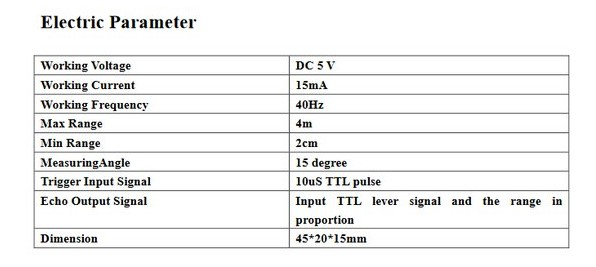
\includegraphics[width=1\linewidth]{Graphics/ultrasonicsensorDatasheet.jpeg}
    \captionof{table}{Ultrasonic Sensor Datasheet}
    \label{fig:enter-label}
\end{figure}
\begin{figure}[h]
    \centering
    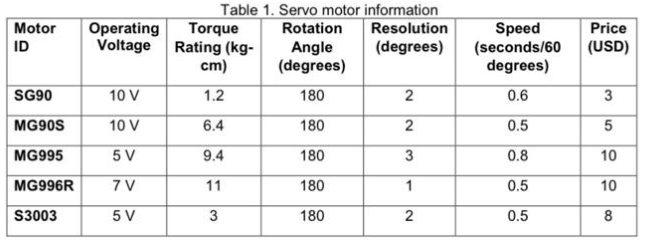
\includegraphics[width=1\linewidth]{servoDatasheeet.png}
    \captionof{table}{Servo Datasheet}
    \label{fig:enter-label}
\end{figure}


\end{document}
